\documentclass[a4paper,11pt]{article}
\usepackage[german]{babel}
\usepackage{hyperref}
%\usepackage[dvips]{graphics}
%\usepackage{graphicx}
\usepackage[pdftex]{graphicx}
\usepackage{amsmath}
\usepackage{amsfonts}
\usepackage{amsthm}
\usepackage{makeidx}
%Formatierung der Fu"snoten
\usepackage[flushmargin]{footmisc}

%\usepackage{myThanks}

% \usepackage{thumbpdf}

\makeindex
\hypersetup{colorlinks=true}

%\newlength{\myFootnoteWidth}
%\newlength{\myFootnoteLabel}
%\setlength{\myFootnoteLabel}{2.2em}%  <-- can be changed to any valid value

\setlength{\textwidth}{460 pt}
\hoffset-0.7in
\newtheorem{definition}{Definition}
\newtheorem{satz}{Satz}
\newenvironment{Beweis}[1]
  {\textbf{Beweis #1} \\}
  {\hfill$\Box$ \\}

%\pdfinfo{ /Title (CrypTool Skript) /Creator (TeX) /Producer
%(pdfTeX 0.14a) /Author (Deutsch Bank AG) /CreationDate
%(D:20000920201000) }


\title{ CrypTool Skript \\ Mathematik und Kryptographie }


\author{
(c) Die Autoren, 1998-2002 \\
Frankfurt am Main \\*[8pt]
}

\begin{document}
\pagestyle{plain}
\setlength{\fboxrule}{.5mm}
\setlength{\fboxsep}{1.75mm}
\setlength{\footnotesep}{6pt}
\addtolength{\footskip}{8pt}
%\setlength{\footskip}{4cm}
%\renewcommand{\footnoterule}{\parindent0cm\rule{13cm}{.1pt}\vspace{.2cm}}
%Formatierung der Fu"snoten

%space between text and footnote 
\renewcommand\footnoterule{%
  \vspace{2em}%   <-- one line space between text and footnoterule
%\kern-3\p@
  \hrule width .4\columnwidth
 \vspace{4pt}
%kern 2.6\p@
}

%\long\def\@makefntext#1{%
%    \parindent 1em%
 %   \noindent
%    \hbox to 1.8em{\hss\@makefnmark}#1}
\maketitle

\parskip 4pt
\vskip + 30 pt
{
In diesem Skript zu dem Programm CrypTool finden Sie eher mathematisch
orientierte Informationen zum Einsatz von
Verschl"usselungsverfahren. Die Hauptkapitel sind von
{\em verschiedenen Autoren} verfa"st und daher in sich abgeschlossen. Am
Ende der meisten Kapitel finden Sie jeweils Literaturangaben und
URL's.

Sie erhalten Informationen "uber die Prinzipien der symmetrischen
und asymmetrischen Verschl"usselung. Ein gro"ser Teil des
Skripts ist dem faszinierenden Thema der Primzahlen gewidmet.
Anhand vieler Beispiele wird in die modulare Arithmetik und die elementare
Zahlentheorie eingef"uhrt, die dann beispielhaft beim RSA-Verfahren
angewandt werden. Danach erhalten Sie Einblick in die mathematischen Ideen
hinter der modernen Kryptographie.

Ein weiteres Kapitel widmet sich kurz den digitalen Signaturen ---
sie sind unverzichtbarer Bestandteil von e-Business Applikationen.
Dazu pa"st das letzte Kapitel: Elliptische Kurven. Die Mathematik der
Elliptischen Kurven ist Grundlage f"ur sehr schnelle kryptographische
Algorithmen zur digitalen Signatur; diese Algorithmen sind f"ur die
Implementierung auf Chipkarten sehr gut geeignet.

W"ahrend das Programm CrypTool eher den praktischen Umgang vermittelt, dient das
Skript dazu, dem an Kryptographie Interessierten ein tieferes Verst"andnis
f"ur die implementierten mathematischen Algorithmen zu vermitteln -- und das didaktisch
m"oglichst gut nachvollziehbar.

Die {\em Autoren} Bernhard Esslinger, Bartol Filipovic, Henrik Koy und
Roger Oyono m"ochten sich an dieser Stelle bedanken bei den Kollegen in der
Firma und an den Universit"aten Frankfurt, Gie"sen und Karlsruhe, insbesondere
bei Dr. Peer Wichmann vom Forschungszentrum Informatik (FZI) Karlsruhe f"ur
die unkomplizierte Unterst"utzung.

% Das Skript dient dazu, dem an Kryptographie Interessierten neben der praktischen
% Anwendung von CrypTool auch ein tieferes Verst"andnis "uber die implementierten
% kryptographischen Algorithmen zu vermitteln.

\enlargethispage{0.5cm}
Wie auch bei CrypTool w"achst die Qualit"at des Skripts mit Ihren Anregungen
und Verbesserungen. Wir freuen uns "uber Ihre R"uckmeldung.


% \begin{tabbing}
% Bernhard Esslinger \= \kill
% Henrik Koy         \>  ({\bf henrik.koy@db.com}) und    \\*[4pt]
% Bernhard Esslinger \> ({\bf bernhard.esslinger@db.com}).
% \end{tabbing}

\vskip +7 pt \noindent
Die aktuelle Version von CrypTool finden Sie unter \newline
  \href{http://www.CrypTool.de}{\tt http://www.CrypTool.de},~~
  \href{http://www.cryptool.com}{\tt http://www.CrypTool.com}~~ oder ~~
  \href{http://www.cryptool.org}{\tt http://www.CrypTool.org}.
\vskip + 7 pt \noindent
Im Readme zu CrypTool sind die Ansprechpartner f"ur dieses kostenlose Tool genannt.
}


\newpage
\tableofcontents
\addcontentsline{toc}{section}{Inhaltsverzeichnis}
\newpage
\normalsize
\parindent0cm
\parskip4pt

% .........................................................................................
%                                      E I N F � H R U N G
% ~~~~~~~~~~~~~~~~~~~~~~~~~~~~~~~~~~~~~~~~~~~~~~~~~~~~~~~~~~~~~~~~~~~~~~~~~~~~~~~~~~~~~~~~~
\section*{Einf"uhrung}  \addcontentsline{toc}{section}{Einf"uhrung}

Dieses Skript wird zusammen mit CrypTool ausgeliefert.

CrypTool ist ein Programm mit sehr umfangreicher Online-Hilfe, mit dessen Hilfe Sie kryptographische Verfahren
anwenden und analysieren k"onnen.\par \vskip + 3pt

F"ur die klassischen Verschl"usselungsverfahren stehen in CrypTool automatische Analysen zur Ver\-f"ugung, die Sie in
die Lage versetzen, mit Kenntnis des verschl"usselten Dokuments und eventuell weiterer Informationen
(unverschl"usseltes Dokument oder Sprache des Dokuments) den Schl"ussel zu ermitteln.\par \vskip + 3pt

CrypTool wurde im Zuge des End-User Awareness Programmes entwickelt, um die Sensibilit"at der
Mitarbeiter f"ur IT-Sicherheit zu erh"ohen und ein tieferes Verst"andnis f"ur den Begriff Sicherheit
zu erm"oglichen.\par \vskip + 3pt

Ein weiteres Anliegen war die Nachvollziehbarkeit der in der Deutschen Bank eingesetzten
kryptographischen Verfahren. So ist es mit CrypTool als verl"a"slicher Referenzimplementierung
der verschiedenen Verschl"usselungsverfahren (aufgrund der Nutzung der Industrie-bew"ahrten \index{SECUDE GmbH} SECUDE-Bibliothek)
auch m"og\-lich, die in anderen Programmen eingesetzte
Verschl"usselung zu testen.\par \vskip + 3pt

Da die Artikel dieses Skripts weitgehend in sich abgeschlossen sind, kann dieses Skript auch unabh"angig
von CrypTool gelesen werden.\par \vskip + 3pt

Die {\em Autoren} haben sich bem"uht, Kryptographie f"ur eine m"oglichst breite Leserschaft darzustellen
-- ohne mathematisch unkorrekt zu werden. Dieser didaktische Anspruch ist am besten geeignet, die Awareness
f"ur die IT-Sicherheit und die Bereitschaft f"ur den Einsatz standardisierter, moderner
Kryptographie zu f"ordern.


% .........................................................................................
%                V E R S C H L U E S S E L U N G S V E R F A H R E N
% ~~~~~~~~~~~~~~~~~~~~~~~~~~~~~~~~~~~~~~~~~~~~~~~~~~~~~~~~~~~~~~~~~~~~~~~~~~~~~~~~~~~~~~~~~
\newpage
\section{Verschl"usselungsverfahren}

\subsection{Verschl"usselung}

Sinn der Verschl"usselung  \index{Verschl""usselung} ist es, Daten so zu ver"andern, dass nur ein autorisierter Empf"an\-ger
in der Lage ist,
den Klartext zu rekonstruieren. Das hat den Vorteil, dass verschl"usselte Daten offen "ubertragen werden
k"onnen und trotzdem keine Gefahr besteht, dass ein Angreifer die Daten unberechtigterweise lesen kann. Der
autorisierte Empf"anger ist im Besitz einer geheimen Information, des sogenannten Schl"ussels, die
es ihm erlaubt, die Daten zu entschl"usseln, w"ahrend sie jedem anderen verborgen bleiben.\par \vskip + 3pt

Es gibt ein beweisbar sicheres Verschl"usselungsverfahren, das \index{One�Time�Pad} {\em One-Time-Pad}. Dieses weist allerdings einige
praktische Nachteile auf (der verwendete Schl"ussel mu"s zuf"allig gew"ahlt werden und genauso lang wie die zu
sch"utzende Nachricht sein), so dass es au"ser in geschlossenen Umgebungen, zum Beispiel beim hei"sen Draht
zwischen Moskau und Washington, kaum eine Rolle spielt.\par \vskip + 3pt

F"ur alle anderen Verfahren gibt es (theoretische) M"oglichkeiten, sie zu brechen. Bei guten Verfahren sind
diese jedoch so aufwendig, dass sie praktisch nicht durchf"uhrbar sind und diese Verfahren als (praktisch)
sicher angesehen werden k"onnen.\par \vskip + 3pt

Grunds"atzlich unterscheidet man zwischen symmetrischen und asymmetrischen Verfahren zur Verschl"usselung.

\subsubsection{Symmetrische Verschl"usselung}

Bei der {\em symmetrischen} Verschl"usselung \index{Verschl""usselung!symmetrisch} m"ussen Sender und Empf"anger "uber einen
gemeinsamen (geheimen)
Schl"ussel verf"ugen, den sie vor Beginn der eigentlichen Kommunikation ausgetauscht haben. Der Sender
benutzt diesen Schl"ussel, um die Nachricht zu verschl"usseln und der Empf"anger, um diese zu entschl"usseln.\par \vskip + 3pt

Vorteile von symmetrischen Algorithmen sind die hohe
Geschwindigkeit, mit denen Daten ver- und entschl"usselt werden.
Ein Nachteil ist das Schl"usselmanagement. Um miteinander
vertraulich kommunizieren zu k"onnen, m"ussen Sender und
Empf"anger vor Beginn der eigentlichen Kommunikation "uber einen
sicheren Kanal einen Schl"ussel ausgetauscht haben. Spontane
Kommunikation zwischen Personen, die sich vorher noch nie begegnet
sind, scheint so nahezu unm"oglich. Soll in einem Netz mit $ n $
Teilnehmern jeder mit jedem zu jeder Zeit spontan kommunizieren
k"onnen, so mu"s jeder Teilnehmer vorher mit jedem anderen der
$n-� 1$ Teilnehmer einen Schl"ussel ausgetauscht haben. Insgesamt
m"ussen also $n(n - 1)/2$ Schl"ussel ausgetauscht werden.\par \vskip + 3pt

Das bekannteste symmetrische Verschl"usselungsverfahren ist der \index{DES} DES--Algorithmus.
Der DES--Algorithmus ist eine Entwicklung von IBM in Zusammenarbeit mit der National Security Agency \index{NSA} (NSA). Er
wurde 1975 als Standard ver"offentlicht. Trotz seines relativ hohen Alters ist jedoch bis heute kein effektiver
Angriff auf ihn gefunden worden. Der effektivste Angriff besteht aus dem Durchprobieren aller m"oglichen
Schl"ussel, bis der richtige gefunden wird ({\em brute--force--attack})\index{Angriff!brute-force}. Aufgrund der relativ kurzen
Schl"ussell"ange von effektiv 56 Bits (64 Bits, die allerdings 8 Parit"atsbits enthalten),
sind in der Vergangenheit schon mehrfach mit dem DES verschl"usselte Nachrichten gebrochen worden, so dass
er heute als nur noch bedingt sicher anzusehen ist. Symmetrische Alternativen zum DES sind zum Beispiel die Algorithmen
IDEA \index{IDEA} oder Triple--DES.\par \vskip + 3pt

Hohe Aktualit"at besitzen die symmetrischen AES-Verfahren. Das
dazu geh"orende Rijndael Verfahren wurde am 2. Oktober 2000 zum
Gewinner des AES-Ausschreibens erkl"art und ist damit Nachfolger
des DES-Verfahrens.

\subsubsection{Asymmetrische Verschl"usselung}

Bei der {\em asymmetrischen} Verschl"usselung \index{Verschl""usselung!asymmetrisch} hat jeder Teilnehmer ein
pers"onliches Schl"us\-selpaar, das aus einem
{\em geheimen} \index{Schl""ussel!geheim} und einem {\em "offentlichen} Schl"ussel \index{Schl""ussel!""offentlich} besteht. Der "offentliche Schl"ussel wird, der Name deutet es an,
"offentlich bekanntgemacht, zum Beispiel in einem Schl"usselverzeichnis im Internet.\par \vskip + 3pt

M"ochte Alice mit Bob kommunizieren, so sucht sie Bobs "offentlichen Schl"ussel aus dem Verzeichnis und benutzt
ihn, um ihre Nachricht an ihn zu verschl"usseln. Diesen verschl"usselten Text schickt sie dann an Bob, der mit
Hilfe seines geheimen Schl"ussels den Text wieder entschl"usseln kann. Da einzig Bob Kenntnis von seinem
geheimen Schl"ussel hat, ist auch nur er in der Lage, an ihn adressierte Nachrichten zu entschl"usseln.
Selbst Alice als Absenderin der Nachricht kann aus der von ihr versandten (verschl"usselten) Nachricht den
Klartext nicht wieder herstellen. Nat"urlich mu"s sichergestellt sein, dass man aus dem "offentlichen
Schl"ussel nicht auf den geheimen Schl"ussel schlie"sen kann.\par \vskip + 3pt

Veranschaulichen kann man sich ein solches Verfahren mit einer
Reihe von einbruchssicheren Briefk"asten. Wenn ich eine Nachricht
verfa"st habe, so suche ich den Briefkasten mit dem Namensschild
des Empf"angers und werfe den Brief dort ein. Danach kann ich die
Nachricht selbst nicht mehr lesen oder ver"andern, da nur der
legitime Empf"anger im Besitz des Schl"ussels f"ur den Briefkasten
ist.\par \vskip + 3pt

Vorteil von asymmetrischen Verfahren ist das einfache
\index{Schl""usselmanagement} Schl"usselmanagement. Betrachten wir
wieder ein Netz mit $n$ Teilnehmern. Um sicherzustellen, dass
jeder Teilnehmer jederzeit eine verschl"usselte Verbindung zu
jedem anderen Teilnehmer aufbauen kann, mu"s jeder Teilnehmer ein
Schl"usselpaar besitzen. Man braucht also $2n$ Schl"ussel oder $n$
Schl"usselpaare. Ferner ist im Vorfeld einer "Ubertragung kein
sicherer Kanal notwendig, da alle Informationen, die zur Aufnahme
einer vertraulichen Kommunikation notwendig sind, offen
"ubertragen werden k"onnen. Hier ist lediglich auf die
Unverf"alschtheit (Integrit"at und Authentizit"at)
\index{Authentizit""at} des "offentlichen Schl"ussels zu achten.
Nachteil: Im Vergleich zu symmetrischen Verfahren sind reine
asymmetrische Verfahren jedoch um ein Vielfaches langsamer.\par \vskip + 3pt

Das bekannteste asymmetrische Verfahren ist der \index{RSA} RSA--Algorithmus,
der nach seinen Entwicklern Ronald \index{Rivest Ronald} Rivest, Adi \index{Shamir Adi} Shamir und Leonard \index{Adleman Leonard} Adleman benannt wurde. Der
RSA--Algorithmus wurde 1978 ver"offentlicht. Das Konzept der asymmetrischen Verschl"usselung wurde erstmals
von Whitfield Diffie \index{Diffie Whitfield}  und Martin \index{Hellman Martin} Hellman in Jahre 1976 vorgestellt. Heute spielen auch die Verfahren nach
ElGamal \index{ElGamal} eine bedeutende Rolle, vor allem die \index{Schnorr} Schnorr--Varianten im \index{DSA} DSA (Digital \index{Signaturen!digitale}Signature Algorithm).

\subsubsection{Hybridverfahren}
\index{Hybridverfahren}
Um die Vorteile von symmetrischen und asymmetrischen Techniken gemeinsam nutzen zu k"onnen, werden
(zur Verschl"usselung) in der Praxis meist Hybridverfahren verwendet.\par \vskip + 3pt

Hier werden die Daten mittels symmetrischer Verfahren
verschl"usselt: der Schl"ussel ist ein vom Absender zuf"allig
generierter Sitzungsschl"ussel (session key)\index{Session Key}, der nur f"ur diese
Nachricht verwendet wird. Anschlie"send wird dieser
Sitzungsschl"ussel mit Hilfe des asymmetrischen Verfahrens
verschl"usselt und zusammen mit der Nachricht an den Empf"anger
"ubertragen. Der Empf"anger kann den Sitzungsschl"ussel mit Hilfe
seines geheimen Schl"ussels bestimmen und mit diesem dann die
Nachricht entschl"usseln. Auf diese Weise nutzt man das bequeme
Schl"usselmanagement \index{Schl""usselmanagement} asymmetrischer
Verfahren und kann trotzdem gro"se Datenmengen schnell und effektiv mit
symmetrischen Verfahren verschl"usseln.

\subsubsection{Weitere Details}

Neben Informationen in der umfangreichen Fachliteratur und im Internet enth"alt auch die 
Online-Hilfe von CrypTool sehr viele details zu den einzelnen symmetrischen und asymmetrischen 
Verschl"usselungsverfahren.

\begin{thebibliography}{99999}
\addcontentsline{toc}{subsection}{Literatur}
\bibitem[Schmeh2001]{Schmeh2001}  \index{Schmeh 2001}
	Klaus Schmeh, \\
	Kryptografie und Public-Key Infrastrukturen im Internet, dpunkt.verlag, 2. akt. und erw. Auflage 2001. \\
	Sehr gut lesbares, hoch aktuelles und umfangreiches Buch "uber Kryptographie. Geht auch auf die praktischen
	Probleme, wie Standardisierung oder real existierende Software, ein.
	Bisher nur in deutsch erschienen.

\end{thebibliography}

% ....................................................................................
%                             P R I M Z A H L E N
% ~~~~~~~~~~~~~~~~~~~~~~~~~~~~~~~~~~~~~~~~~~~~~~~~~~~~~~~~~~~~~~~~~~~~~~~~~~~~~~~~~~~~
\newpage
\section{Primzahlen}
(Bernhard Esslinger, besslinger@web.de, Mai 1999, Updates Nov. 2000, Dezember 2001)
\hypertarget{Kapitel_2}{}

%\paragraph{Was sind Primzahlen?}
\subsection*{Was sind Primzahlen?}
\addcontentsline{toc}{subsection}{~~~~~~Was sind Primzahlen?}
\index{Primzahlen} \index{Zahlen!Primzahl} Primzahlen sind ganze,
positive Zahlen gr"o"ser gleich $2$, die man nur durch 1 und durch
sich selbst teilen kann. Alle anderen nat"urlichen Zahlen gr"o"ser
gleich $2$ lassen sich durch Multiplikation von Primzahlen
bilden.

Somit bestehen die {\em nat"urlichen} \index{Zahlen} Zahlen $ \mathbb{N} = \{1, 2,
3, 4,\cdots \} $ aus
\begin{itemize}
   \item der Zahl $1$ (dem Einheitswert)
   \item den Primzahlen (primes) und
   \item den zusammengesetzten Zahlen (composite numbers).
\end{itemize}

Primzahlen haben aus 3 Gr"unden besondere Bedeutung erlangt:
\begin{itemize}
  \item Sie werden in der Zahlentheorie als die Grundbausteine der nat"urlichen Zahlen betrachtet,
        anhand derer eine Menge genialer mathematischer "Uberlegungen gef"uhrt wurden.
  \item Sie haben in der modernen \index{Kryptographie!moderne} Kryptographie (Public Key \index{Kryptographie!Public Key} Kryptographie) gro"se praktische
        Bedeutung erlangt. Das verbreitetste Public Key Verfahren ist die Ende der siebziger Jahre
        erfundene \index{RSA} RSA-Verschl"usselung. Nur die Verwendung (gro"ser) Primzahlen f"ur bestimmte
        Parameter garantiert die Sicherheit des Algorithmus sowohl beim RSA-Verfahren als auch bei
        noch moderneren Verfahren (digitale \index{Signaturen!digitale} Signatur, Elliptische Kurven).
  \item Die Suche nach den gr"o"sten bekannten Primzahlen hat wohl bisher keine praktische
        Verwendung, erfordert aber die besten Rechner, gilt als hervorragender Benchmark (M"oglichkeit
        zur Leistungsbestimmung von Computern) und f"uhrt zu neuen Formen der Berechnungen auf
        mehreren Computern \\
        (siehe auch: \href{http://www.mersenne.org/prime.htm}{\tt http://www.mersenne.org/prime.htm}).
\end{itemize}
Von Primzahlen lie"sen sich im Laufe der letzten zwei Jahrtausende sehr viele Menschen faszinieren.
Der Ehrgeiz, zu neuen Erkenntnissen "uber Primzahlen zu gelangen, f"uhrte dabei oft zu genialen Ideen
und Schlu"sfolgerungen.
Im folgenden wird in einer leicht verst"andlichen Art in die mathematischen Grundlagen der Primzahlen
eingef"uhrt. Dabei kl"aren wir auch, was "uber die Verteilung (Dichte, Anzahl von Primzahl in einem
bestimmten Intervall) der Primzahlen bekannt ist oder wie Primzahltests funktionieren.

% -----------------------------------------------------------------------------------------------------------------------
\subsection{Primzahlen in der Mathematik}

Jede ganze Zahl hat Teiler. Die Zahl 1 hat nur einen, n"amlich
sich selbst. Die Zahl $12$ hat die sechs Teiler $1, 2, 3, 4, 6,
12$. Viele Zahlen sind nur teilbar durch sich selbst und durch
$1$. Bez"uglich der Multiplikation sind dies die \glqq Atome\grqq
~ im Bereich der Zahlen. Diese Zahlen nennt man Primzahlen.

In der Mathematik ist eine etwas andere (aber "aquivalente) Definition "ublich.

% \begin{definition}
% Eine ganze Zahl $p > 1$ hei"st \index{Zahlen!Primzahl} Primzahl, wenn f"ur alle ganze Zahlen $a$ und $b$ gilt:
% wenn $p$ weder $a$ noch $b$ teilt, dann teilt $p$ auch nicht die Zahl $a\cdot b$.
% \end{definition}
\begin{definition}\label{def-pz-prime}
Eine ganze Zahl $p \in {\bf N}$ hei"st Primzahl \index{Zahlen!Primzahl}, wenn $p > 1$ und $p$ nur die trivialen
Teiler $\pm 1$ und $\pm p$ besitzt.
\end{definition}


Per definitionem ist die Zahl $1$ keine Primzahl. Im weiteren bezeichnet der Buchstabe $p$ stets eine Primzahl.

Die Primzahlenfolge startet mit
$$ 2,~ 3,~ 5,~ 7, ~ 11, ~ 13, ~ 17, ~ 19, ~ 23, ~ 29, ~ 31, ~ 37, ~ 41, ~ 43, ~ 47, ~ 53, ~ 59, ~ 61, ~ 67, ~ 71, ~ 73, ~ 79, ~ 83, ~ 89, ~ 97, \cdots .$$
Unter den ersten 100 Zahlen gibt es genau 25 Primzahlen. Danach nimmt ihr prozentualer Anteil stets
ab. Primzahlen k"onnen nur auf eine einzige {\em triviale} Weise zerlegt werden:
$$5 = 1 \cdot 5,\quad  17 = 1 \cdot 17, \quad 1013 = 1 \cdot 1.013,  \quad 1.296.409 = 1 \cdot 1.296.409.$$
Alle Zahlen, die $2$ und mehr Faktoren haben, nennt man \index{Zahlen!zusammengesetzte} {\em zusammengesetzte}. Dazu geh"oren
$$ 4 = 2 \cdot 2, \quad 6 = 2\cdot 3 $$
aber auch Zahlen, die {\em wie Primzahlen aussehen}, aber doch keine sind:
$$ 91 = 7 \cdot 13, \quad 161=7 \cdot 23, \quad 767 =13 \cdot 59. $$

\begin{satz}\label{thm-pz-sqr}
Jede ganze Zahl $m$ gr"o"ser als $1$ besitzt einen kleinsten Teiler gr"o"ser als $1$.
Dieser ist eine Primzahl $p$. Sofern $m$ nicht selbst eine Primzahl ist, gilt:
$p$ ist kleiner oder gleich der Quadratwurzel aus $m$.
\end{satz}

Aus den Primzahlen lassen sich alle ganzen Zahlen gr"o"ser als $1$ zusammensetzen --- und das sogar in
einer eindeutigen Weise. Dies besagt der 1. Hauptsatz der Zahlentheorie (= Hauptsatz der elementaren Zahlentheorie =
fundamental theorem of arithmetic = fundamental building block of all positive integers).\index{Zahlentheorie!Hauptsatz}

\begin{satz}\label{thm-pz-prod}
Jedes Element $n$ gr"o"ser als $1$ der nat"urlichen Zahlen l"a"st sich als Produkt
$n = p_1 \cdot p_2 \dots p_m$ von Primzahlen schreiben.
Sind zwei solche Zerlegungen
$$n =  p_1 \cdot p_2 \cdots p_m = p'_1 \cdot p'_2 \cdots p'_{m'}$$
gegeben, dann gilt nach eventuellem Umsortieren $\;m = m'\;$ und  f"ur alle $i$:  $\;p_i = p'_i$.
\end{satz}

In anderen Worten: Jede nat"urliche Zahl au"ser der $1$ l"a"st sich auf genau eine Weise als Produkt von
Primzahlen schreiben, wenn man von der Reihenfolge der Faktoren absieht. Die Faktoren sind also
eindeutig (die {\em Expansion in Faktoren} ist eindeutig)!
Zum Beispiel ist
$$ 60 = 2 \cdot 2 \cdot 3 \cdot 5 = 2^2\cdot 3^1 \cdot 5^1 $$
Und das ist --- bis auf eine ver"anderte Reihenfolge der Faktoren
--- die einzige M"oglichkeit, die Zahl $60$ in Primfaktoren zu
zerlegen. Wenn man nicht nur Primzahlen als Faktoren zul"a"st,
gibt es mehrere M"oglichkeiten der Zerlegung in Faktoren und die
Eindeutigkeit (uniqueness) geht verloren: \hypertarget{uniqueness}{}
$$ 60 = 1 \cdot 60 = 2 \cdot 30 = 4 \cdot 15 = 5 \cdot 12 =6 \cdot 10 = 2 \cdot 3 \cdot 10 =
        2 \cdot 5 \cdot 6 = 3 \cdot 4 \cdot 5 = \cdots . $$

Der folgende Absatz wendet sich eher an die mit der mathematischen Logik vertrauteren Menschen:
Der 1. Hauptsatz ist nur scheinbar selbstverst"andlich\label{remFundTheoOfArithm}. Man kann viele andere Zahlenmengen
(ungleich der positiven ganzen Zahlen gr"o"ser als 1) konstruieren, bei denen selbst eine Zerlegung in
die Primfaktoren dieser Mengen nicht eindeutig ist:
In der Menge $M = \{1, 5, 10, 15, 20, \cdots\}$ gibt es unter der Multiplikation kein Analogon zum Hauptsatz.
Die ersten f"unf Primzahlen dieser Folge sind $5, 10, 15, 20, 30$ (beachte: $10$ ist prim, da innerhalb
dieser Menge $5$ kein Teiler von $10$ ist --- das Ergebnis $2$ ist kein Element der gegebenen Grundmenge
$M$). Da in $M$ gilt:
$$ 100 = 5 \cdot 20 = 10 \cdot 10 $$
und sowohl $5, 10, 20$ Primzahlen dieser Menge sind, ist hier die Zerlegung in Primfaktoren nicht
eindeutig.

% ---------------------------------------------------------------------------------------------------------------------------
\subsection{Wie viele Primzahlen gibt es?}

F"ur die nat"urlichen Zahlen sind die Primzahlen vergleichbar mit den Elementen in der Chemie oder
den Elementarteilchen in der Physik (vgl. \cite[S. 22]{Blum1999}).

W"ahrend es nur $92$ nat"urliche chemische Elemente gibt, ist die Anzahl der Primzahlen unbegrenzt.
Das wu"ste schon der Grieche \index{Euklid} Euklid\footnote{Euklid, griechischer Mathematiker des 4./3. Jahrhunderts vor Christus.
Wirkte an der Akademie in Alexandria und verfa"ste mit den \glqq Elementen\grqq~ das bekannteste systematische Lehrbuch
der griechischen Mathematik.} im dritten vorchristlichen Jahrhundert.
\begin{satz}[Euklid]\label{thm-pz-euklid}\footnote{Die "ublich gewordene Benennung soll nicht sagen,
dass Euklid der Entdecker des Satzes ist, da dieser
nicht bekannt ist. Der Satz wird bereits in Eulkids \glqq Elementen\grqq ~(Buch IX, Satz 20) 
formuliert und bewiesen. Die dortige Formulierung ist insofern bemerkenswert,
als sie das Wort \glqq unendlich\grqq~ nicht verwendet; sie lautet
$$
O\acute{\iota}~\pi\varrho\tilde{\omega}\tau o \iota~\grave{\alpha}\varrho\iota\vartheta\mu o\grave{\iota}~
\pi\lambda\varepsilon\acute{\iota}o \upsilon\varsigma~\varepsilon\grave{\iota}\sigma\grave{\iota}~
\pi\alpha\nu\tau\grave{o}\varsigma~\tau o \tilde{\upsilon}~
\pi\varrho o \tau\varepsilon\vartheta\acute{\varepsilon}\nu\tau o \varsigma~
\pi\lambda\acute{\eta}\vartheta\ o \upsilon\varsigma~
\pi\varrho\acute{\omega}\tau\omega\nu~
\grave{\alpha}\varrho\iota\vartheta\mu\tilde{\omega}\nu,
$$
zu deutsch: Die Primzahlen sind mehr als jede vorgegebene Menge von Primzahlen.}
Die Folge der Primzahlen bricht nicht ab, es gibt also unendlich viele Primzahlen.
\end{satz}

Sein Beweis, dass es
unendlich viele Primzahlen gibt, gilt bis heute als ein Glanzst"uck mathematischer "Uberlegung und
Schlu"sfolgerung (Widerspruchsbeweis). Er nahm an, es gebe nur endlich viele Primzahlen und damit
eine gr"o"ste Primzahl. Daraus zog er solange logische Schl"usse, bis er auf einen offensichtlichen
Widerspruch stie"s. Damit mu"ste etwas falsch sein. Da sich in die Schlu"skette kein Lapsus
eingeschlichen hatte, konnte es nur die Annahme sein. Demnach mu"ste es unendlich viele
Primzahlen geben!

\hypertarget{euklid}{}
\paragraph{Euklid's Widerspruchsbeweis}\index{Euklid's Widerspruchsbeweis}
f"uhrt die Argumentation wie folgt:

{\bf Annahme:} \quad Es gibt {\em endlich} viele Primzahlen.
\\*[4pt] {\bf Schlu"s:} \quad Dann lassen sie sich auflisten $p_1
< p_2 < p_3 < \dots < p_n$, wobei $n$ f"ur die (endliche) Anzahl
der Primzahlen steht. $p_n$ w"are also die gr"o"ste Primzahl. Nun
betrachtet Euklid die Zahl $a = p_1 \cdot p_2 \cdots p_n +1$.
Diese Zahl kann keine Primzahl sein, da sie in unserer
Primzahlenliste nicht auftaucht. Also mu"s sie durch eine Primzahl
teilbar sein. D.h. es gibt eine nat"urliche Zahl $i$ zwischen $1$
und $n$, so dass $p_i$ die Zahl $a$ teilt. Nat"urlich teilt $p_i$
auch das Produkt $a-1 = p_1 \cdot p_2 \cdots p_n$, da $p_i$ ja ein
Faktor von $a-1$ ist. Da $ p_i $ die Zahlen $ a $ und $ a-1 $
teilt, teilt sie auch die Differenz dieser Zahlen. Daraus folgt:
$p_i$ teilt  $a - (a-1) = 1$. $p_i$ m"u"ste also $1$ teilen und
das ist unm"oglich.\\*[4pt] 
{\bf Wiederspruch}: \quad Unsere Annahme war falsch.\par
Also gibt es {\em unendlich} viele Primzahlen
\hyperlink{primhfk}{(Verweis: "Ubersicht unter 2.6.1 "uber die
Anzahl von Primzahlen in verschiedenen Intervallen).}\par \vskip + 3pt

Wir erw"ahnen hier auch noch eine andere, auf den ersten Blick "uberraschende Tatsache, dass n"amlich in der
Folge aller Primzahlen $p_1, p_2, \cdots $ L"ucken von beliebig gro"ser L"ange $n$ auftreten. Unter den $n$ aufeinanderfolgenden
 nat"urlichen Zahlen
$$ (n+1)!+2, \cdots, (n+1)!+(n+1),
$$
ist keine eine Primzahl, da ja in ihnen der Reihe nach die Zahlen $2,\cdots, n+1$ als echte Teiler enthalten sind
(Dabei bedeutet $n!$ das Produkt der ersten $n$ nat"urlichen Zahlen, also 
$n!=n*(n-1)* \cdots *3*2*1$). 
% ---------------------------------------------------------------------------------------------------------------------
\subsection{Die Suche nach sehr gro"sen Primzahlen}

Die gr"o"sten heute bekannten Primzahlen haben mehrere
hunderttausend Stellen. Das ist unvorstellbar gro"s. Die Anzahl
der Elementarteilchen im Universum wird auf \glqq nur\grqq\ eine
$80$-stellige Zahl gesch"atzt \hyperlink{grosord}{(Verweis:
"Ubersicht unter 2.6.3 "uber verschiedene Gr"o"senordnungen /
Dimensionen)}.

Nahezu alle bekannten riesig gro"sen Primzahlen sind spezielle Kandidaten, sogenannte \index{Mersenne Marine}
{\em Mersennezahlen} der Form $2^p -1,$
wobei $p$ eine Primzahl ist. Marin Mersenne (1588-1648) war ein franz"osicher Priester und
Mathematiker. Nicht alle Mersennezahlen sind prim:
$$
\begin{array}{cl}
2^2 - 1 = 3 & \Rightarrow {\rm prim} \\
2^3 - 1 = 7 & \Rightarrow {\rm prim} \\
2^5 - 1 = 31    & \Rightarrow {\rm prim} \\
   \vdots        \\
2^{11} - 1 = 2.047 = 23 \cdot 89    & \Rightarrow  {\rm NICHT~prim} !
\end{array}
$$

\index{Zahlen!Mersennezahlen}\index{Mersenne Marine!Mersennezahlen} \index{Mersenne Marine!Satz} 
Dass Mersennezahlen nicht immer Primzahlen (Mersenne-Primzahlen) sind, wu"ste auch schon Mersenne (siehe Exponent $p = 11$).
Dennoch ist ihm der interessante Zusammenhang zu verdanken, dass eine Zahl der Form $2^n-1$
keine Primzahl ist, wenn $n$ eine zusammengesetzte Zahl ist:

\begin{satz}[Mersenne]\label{thm-pz-mersenne}
Wenn $2^n - 1$ eine Primzahl ist, dann folgt, $n$ ist ebenfalls
eine Primzahl.
\end{satz}

\begin{Beweis}{}
Der Beweis des Satzes von Mersenne kann durch Widerspruch
durchgef"uhrt werden. Wir nehmen also an, dass es eine
zusammengesetzte nat"urliche Zahl $ n $ (mit echter Zerlegung)  $
n=n_1 n_2 $ gibt, mit der Eigenschaft, dass $ 2^n -1 $ eine
Primzahl ist.

Wegen
\begin{eqnarray*}
(x^r-1)((x^r)^{s-1} + (x^r)^{s-2} + \cdots + x^r +1) & = &  ((x^r)^s + (x^r)^{s-1} + (x^r)^{s-2} + \cdots + x^r) \\
&  & -((x^r)^{s-1} + (x^r)^{s-2} + \cdots + x^r +1)  \\
& = & (x^r)^s -1 = x^{rs } -1,
\end{eqnarray*}
folgt
\[ 2^{n_1 n_2} - 1 = (2^{n_1} -1)((2^{n_1})^{n_2 -1} + (2^{n_1})^{n_2 -2} + \cdots + 2^{n_1} + 1). \]
Da $ 2^n - 1 $ eine Primzahl ist, mu"s einer der obigen beiden
Faktoren auf der rechte Seite gleich 1 sein. Dies kann nur dann
der Fall sein, wenn $ n_1 =1 $ oder $ n_2 =1$ ist. Dies ist aber
ein Widerspruch unserer Annahme. Deshalb ist unsere Annahme
falsch. Also gibt es keine zusammengesetzte Zahl $ n, $ so dass $
2^n -1 $ eine Primzahl ist.
\end{Beweis} \vskip + 5pt
Leider gilt dieser Satz nur in einer Richtung (die Umkehrung gilt
nicht, keine "Aquivalenz): siehe das obige Beispiel $2^{11}-1, $
wo $11$ prim ist.

Mersenne behauptete, dass $2^{67}-1$ eine Primzahl ist. Auch zu
dieser Behauptung gibt es mathematisch eine interessante Historie:
Zuerst dauerte es "uber 200 Jahre, bis \index{Lucas Edouard}
Edouard Lucas (1842-1891) bewies, dass diese Zahl zusammengesetzt
ist. Er argumentierte aber indirekt und kannte keinen der
Faktoren. Dann zeigte Frank Nelson 1903, aus welchen Faktoren,
diese Primzahl besteht:
$$ 2^{67} -1 =147. 573. 952. 588. 676. 412. 927 = 193. 707. 721 \cdot 761. 838. 257. 287. $$
Er gestand, 20 Jahre an der Faktorisierung (Zerlegung in Faktoren)
dieser 21-stelligen Dezimalzahl gearbeitet zu haben!

Dadurch, dass man bei den Exponenten der Mersennezahlen nicht alle nat"urlichen Zahlen verwendet,
sondern nur die Primzahlen, engt man den {\em Versuchsraum} deutlich ein.
Die derzeit bekannten Mersenne-Primzahlen gibt es f"ur die Exponenten
$$
\begin{array}{c}
2, ~ 3, ~ 5, ~ 7, ~ 13, ~ 17, ~ 19, ~ 31, ~ 61, ~ 89, ~ 107, ~ 127, ~ 521, ~ 607, ~ 1.279, ~ 2.203, ~ 2.281, ~ 3.217, ~ 4.253, ~ 4.423, \\
9.689, ~ 9.941, ~ 11.213, ~ 19.937, ~ 21.701, ~ 23.207, ~ 44.497, ~ 86.243, ~ 110.503, ~ 132.049, ~ 216.091,\\
 756.839, ~ 859.433, ~ 1.257.787, ~ 1.398.269, ~ 2.976.221, ~ 3.021.377, ~ 6.972.593, ~13.466.917.
\end{array}
$$
Damit sind heute $39$ Mersenne-Primzahlen bekannt.

Die $19$. Zahl
mit dem Exponenten $4.253$ war die erste mit mindestens $1.000$
Stellen im Zehnersystem (der Mathematiker Samual \index{Yates
Samual} Yates pr"agte daf"ur den Ausdruck {\em titanische}
\index{Primzahlen!titanische} Primzahl; sie wurde 1961 von Hurwitz
gefunden); die $27$. Zahl mit dem Exponenten $44.497$ war die
erste mit mindestens $10.000$ Stellen im Zehnersystem (Yates
pr"agte daf"ur den Ausdruck \index{Primzahlen!gigantische}  {\em
gigantische} Primzahl. Diese Bezeichnungen sind heute l"angst
veraltet).

Die 37. Zahl wurde im Januar 1998 gefunden und hat
909.526 Stellen im Zehnersystem, was 33 Seiten in der FAZ
entspricht!

Man findet diese Zahlen unter den URLs

{\href{http://reality.sgi.com/chongo/prime/prime_press.html}{\tt
http://reality.sgi.com/chongo/prime/prime\_press.html}}
\vskip - 4pt \noindent
\begin{quote}
(Der Supercomputerhersteller SGI Cray Research besch"aftigte nicht
nur hervorragende Mathematiker, sondern benutzte die Primzahltests
auch als Benchmarks f"ur seine Maschinen.)
\end{quote}
{\href{http://www.utm.edu/}{\tt http://www.utm.edu/}}
\vskip - 4pt \noindent
\begin{quote}
(An der Universit"at von Tennessee findet man umfangreiche Forschungsergebnisse "uber Primzahlen.)
\end{quote}

\subsubsection{M-38 -- Juni 1999} \index{Mersenne Marine!M-38}
Die 38. Mersenne-Primzahl, genannt M-38, $$ 2^{6.972.593} - 1 $$
wurde im Juni 1999 gefunden und hat $2.098.960$ Stellen im
Zehnersystem (das entspricht rund 77 Seiten in der FAZ).
\subsubsection{M-39 -- Dezember 2001}\index{Mersenne Marine!M-39}
Die 39. Mersenne-Primzahl, genannt M-39, $$2^{13.466.917}-1$$  wurde am 6.12.2001 gefunden -- genau
genommen war am 6.12.2001 die Verifikation der am 14.11.2001 von dem kanadischen Studenten Michael Cameron gefundenen Primzahl abgeschlossen.
Diese Zahl hat rund 4 Millionen Stellen (genau 4.053.946 Stellen). Allein zu ihrer Darstellung
($924947738006701322247758 \cdots 1130073855470256259071$) br"auchte man in der FAZ knapp 200 Seiten.
\subsubsection{GIMPS}\index{GIMPS}
Mit der 39. Mersenne-Primzahl hat das 1996 gegr"undete GIMPS-Projekt (Great Internet Mersenne-Prime Search) bereits
zum 5. Mal die gr"o"ste Mersenne-Zahl entdeckt, die erwiesenerma"sen prim ist.

Am GIMPS-Projekt beteiligen sich z.Zt. rund 130.000 freiwillige Amateure und Experten, die ihre Rechner in das
von der Firma entropia organisierte \glqq primenet\grqq~ einbinden, um mit verteilten Computerprogrammen solche Zahlen zu finden.
\subsubsection{EFF}\index{EFF}

Angefacht wird diese Suche noch zus"atzlich durch einen Wettbewerb, den die Non\-profit-Organisation
EFF (Electronic Frontier Foundation) mit den Mitteln eines unbekannten Spenders gestartet hat. Den
Teilnehmern winken Gewinne im Gesamtwert von 500.000 USD, wenn sie die l"angste Primzahl
finden. Dabei sucht der unbekannte Spender nicht nach dem schnellsten Rechner, sondern er will auf
die M"oglichkeiten des {\em cooperative networking} aufmerksam machen

{\href{http://www.eff.org/coopawards/prime-release1.html}{\tt http://www.eff.org/coopawards/prime-release1.html}}.

Der Entdecker von M-38 erhielt f"ur die Entdeckung der ersten Primzahl mit "uber 1 Million Dezimalstellen von der EFF eine
Pr"amie von 50.000 USD. Die n"achste Pr"amie von 100.000 USD gibt es von der EFF f"ur eine Primzahl mit mehr als 10 Millionen
Dezimalstellen.
% {\href{http://www.octocad.demon.co.uk/mersenne/prime.htm}{\tt http://www.octocad.demon.co.uk/mersenne/prime.htm}}.

Edouard Lucas (1842-1891) hielt "uber 70 Jahre den Rekord der gr"o"sten bekannten Primzahl, indem
er nachwies, dass $2^{127}-1$ prim ist. Solange wird wohl kein neuer Rekord mehr Bestand haben.

% ----------------------------------------------------------------------------------------------------------------------------
\subsubsection{Primzahltests}
\index{Primzahltest}
F"ur die Anwendung sicherer Verschl"usselungsverfahren braucht man sehr gro"se Primzahlen (im
Bereich von $2^{2.048}$, das sind Zahlen im Zehnersystem mit "uber $600$ Stellen!).

Bisher haben wir immer nach den Primfaktoren gesucht, um zu entscheiden, ob eine Zahl prim ist.
Wenn aber auch der kleinste Primfaktor riesig ist, dauert die Suche zu lange. Die Zerlegung in
Faktoren mittels rechnerischer systematischer Teilung oder mit dem Sieb des Eratosthenes (siehe
unten) ist mit heutigen Computern anwendbar f"ur Zahlen mit bis zu circa $20$ Stellen im Zehnersystem.

Ist aber etwas "uber die {\em Bauart} der fraglichen Zahl bekannt, gibt es sehr hochentwickelte Verfahren,
die deutlich schneller sind.
Fermat\index{Fermat} hatte im 17. Jahrhundert an Mersenne geschrieben, dass er vermute, dass alle Zahlen der Form
$$ F(n) = 2^{2^n} + 1 $$
f"ur alle ganzen Zahlen $n$ gr"o"ser oder gleich $0$ prim seien (siehe unten).

Schon im 19. Jahrhundert wu"ste man, dass die $29$-stellige Zahl
$$ F(7) = 2^{2^7} + 1 $$
keine Primzahl ist. Aber erst 1970 fanden Morrison/Billhart ihre Zerlegung.
\begin{eqnarray*}
F(7) & = & 34.279.974.696.877.740.253.374.607.431.768.211.457 \\
& = & 59. 649. 589. 127. 497. 217 \cdot  574. 689. 200. 685.
129.054. 721.
\end{eqnarray*}
Der Ausgangspunkt vieler schneller Primzahltests ist der (kleine)
Fermatsche Satz, den Fermat im Jahr 1640 aufstellte.
\index{Fermat!kleiner Fermat}
\begin{satz}[\glqq kleiner\grqq\ Fermat]\label{thm-pz-fermat1}
Sei $p$ eine Primzahl und $a$ eine beliebige ganze Zahl, dann gilt f"ur alle $a$
$$a^p \equiv a \; {\rm mod} \; p.$$
Eine alternative Formulierung lautet: \\
Sei $p$ eine Primzahl und $a$ eine beliebige ganze Zahl, die kein
Vielfaches von $p$ ist (also $a \not\equiv 0 \; {\rm mod} \; p$),
dann gilt $a^{p-1} \equiv 1 \; {\rm mod} \; p$.
\end{satz}

Wer mit dem Rechnen mit Resten (Modulo-Rechnung) nicht so vertraut ist, m"oge den Satz einfach so
hinnehmen oder \hyperlink{Kapitel_3}{Kapitel 3 \glqq Einf"uhrung in die
elementare Zahlentheorie mit Beispielen\grqq} lesen. Wichtig ist, dass aus diesem Satz folgt, dass wenn diese Gleichheit f"ur irgendein ganzes $a$
nicht erf"ullt ist, dann ist $p$ keine Primzahl! Die Tests lassen sich (zum Beispiel f"ur die erste
Formulierung) leicht mit der {\em Testbasis} $a = 2$ durchf"uhren.

Damit hat man ein Kriterium f"ur Nicht-Primzahlen, also einen negativen Test, aber noch keinen
Beweis, dass eine Zahl $a$ prim ist.
Leider gilt die Umkehrung zum Fermatschen Satz nicht, sonst h"atten wir einen einfachen Beweis f"ur
die Primzahleigenschaft (man sagt auch, man h"atte dann ein einfaches Primzahlkriterium).

Anmerkung: Zahlen, die die Eigenschaft
$$ 2^n \equiv 2 \;{\rm mod}\; n $$
erf"ullen, aber nicht prim sind, bezeichnet man als \index{Pseudoprimzahlen}\index{Zahlen!Pseudoprimzahl} {\em Pseudoprimzahlen}.
Die erste Pseudoprimzahl (also keine Primzahl) ist
$$ 341 = 11 \cdot 31. $$
Es gibt Zahlen, die den Fermat-Test mit allen Basen bestehen und doch nicht prim sind: diese Zahlen
hei"sen \index{Zahlen!Carmichael Zahlen} {\em Carmichael-Zahlen}. Die erste ist
$$ 561 = 3 \cdot 11 \cdot 17. $$
Ein st"arkerer Test stammt von \index{Miller} \index{Rabin}
Miller/Rabin: er wird nur von sogenannten {\em starken
Pseudoprimzahlen} bestanden. Wiederum gibt es starke
Pseudoprimzahlen, die keine Primzahlen sind, aber das passiert
deutlich seltener als bei den (einfachen) Pseudoprimzahlen. Die
kleinste starke Pseudoprimzahl zur Basis $2$ ist
$$ 15.841 = 7 \cdot 31 \cdot 73. $$
Testet man alle 4 Basen $2, 3, 5$ und $7$ findet man bis $25 \cdot 10^9$
nur eine starke Pseudoprimzahl, also eine Zahl, die den Test besteht und doch keine Primzahl ist.

Weiterf"uhrende Mathematik hinter dem Rabin-Test gibt dann die Wahrscheinlichkeit an, mit der die
untersuchte Zahl prim ist (solche Wahrscheinlichkeiten liegen heutzutage bei circa  $10^{-60}$).

Ausf"uhrliche Beschreibungen zu Tests, um herauszufinden, ob eine Zahl prim ist, finden sich zum
Beispiel unter:

{\href{http://www.utm.edu/research/primes/mersenne.shtml}{\tt http://www.utm.edu/research/primes/mersenne.shtml}} und

{\href{http://www.utm.edu/research/primes/prove/index.html}{\tt
http://www.utm.edu/research/primes/prove/index.html}}.



% --------------------------------------------------------------------------------------------------------
\subsection{Die Suche nach einer Formel f"ur Primzahlen}
\index{Primzahlen!Formel}
Derzeit sind keine brauchbaren, offenen (also nicht rekursiven) Formeln bekannt, die nur Primzahlen
liefern (rekursiv bedeutet, dass zur Berechnung der Funktion auf dieselbe Funktion in Abh"angigkeit
einer kleineren Variablen zugegriffen wird). Die Mathematiker w"aren schon zufrieden, wenn sie eine
Formel f"anden, die wohl L"ucken l"a"st (also nicht alle Primzahlen liefert), aber sonst keine
zusammengesetzten Zahlen (Nichtprimzahlen) liefert.

Optimal w"are, man w"urde f"ur das Argument $n$ sofort die $n$-te Primzahl bekommen, also f"ur
$f(8) = 19\,$ oder f"ur  $f(52) = 239$.

Ideen dazu finden sich in

{\href{http://www.utm.edu/research/primes/notes/faq/p_n.html}{\tt http://www.utm.edu/research/primes/notes/faq/p\_n.html}}.

Verweis: \hyperlink{ntePrimzahl}{Die Tabelle unter 2.6.2} enth"alt  die exakten Werte f"ur
die $n$-ten Primzahlen f"ur ausgew"ahlte $ n.$
%Es gibt eine Tabelle mit exakten Werten f"ur die n-ten Primzahlen f"ur bestimmte $n$.

Im folgenden einige der verbreitetsten Ans"atze f"ur
Primzahlformeln:
\begin{enumerate}
  \item Mersennezahlen  $f(n) = 2^n - 1$: \\
    Wie oben gesehen, liefert diese Formel wohl relativ viele gro"se Primzahlen, aber es kommt -- wie
    f"ur $n=11$ [$f(n)=2.047$] -- immer wieder vor, dass das Ergebnis nicht prim ist.
  \item $F(k,n) = k \cdot 2^n \pm 1$  f"ur $ n $ prim und $ k $ kleine Primzahlen:\\
   F"ur diese Verallgemeinerung der Mersennezahlen gibt es (f"ur kleine $k$) ebenfalls sehr schnelle
    Primzahltests (vgl. \cite{Knuth1981}).
    Praktisch ausf"uhren l"a"st sich das zum Beispiel mit der Software PROTHS von Yves Gallot

    ({\href{http://www.prothsearch.net/index.html}
          {\tt http://www.prothsearch.net/index.html}}).
  \item {\em Fermatzahlen}\footnote{Die Fermatschen Primzahlen spielen unter anderem eine wichtige Rolle in der Kreisteilung. Wie Gau"s
\index{Gauss} bewiesen hat, ist das regul"are $p$-Eck f"ur eine Primzahl $p>2$ dann und nur dann mit Zirkel und
Lineal konstruierbar, wenn $p$ eine Fermatsche Primzahl ist.}
\index{Zahlen!Fermatzahlen}\index{Fermat!Fermatzahl}  $F(n) = 2^{2^n} + 1$:\\
    Wie oben erw"ahnt, schrieb Fermat diese Vermutung an Mersenne. Erstaunlicherweise w"are es f"ur
    ihn m"oglich gewesen, mit dem auf seinem kleinen Satz beruhenden negativen Primzahltest f"ur
    $n=5$  ein positives Ergebnis zu erhalten.
$$
\begin{array}{lll}
F(0) = 2^{2^0} + 1  = 2^1 + 1 & = 3 &   \mapsto {\rm ~prim}  \\
F(1) = 2^{2^1} + 1  = 2^2 + 1 & = 5 &   \mapsto {\rm ~prim}  \\
F(2) = 2^{2^2} + 1  = 2^4 + 1 & = 17 &  \mapsto {\rm ~prim}  \\
F(3) = 2^{2^3} + 1  = 2^8 + 1 & = 257 & \mapsto {\rm ~prim}  \\
F(4) = 2^{2^4} + 1  = 2^{16} + 1 &  = 65.537 &  \mapsto {\rm ~prim}  \\
F(5) = 2^{2^5} + 1  = 2^{32} + 1 &  = 4 .294. 967. 297 = 641 \cdot
6.700.417 &  \mapsto {\rm ~NICHT~prim} !
\end{array}
$$
  \item Carmichaelzahlen: s.o.
  \item Pseudoprimzahlen: s.o.
  \item starke Pseudoprimzahlen: s.o.
  \item Idee aufgrund von \hyperlink{euclid}{Euklids Beweis} (unendlich viele Primzahlen)
        $p_1 \cdot p_2 \cdots p_n +1$:
$$
\begin{array}{lll}
2{\cdot}3 +1 &      = 7 &          \mapsto {\rm ~prim} \\
2{\cdot}3{\cdot}5 +1 &      = 31    &      \mapsto {\rm ~prim} \\
2{\cdot}3{\cdot}5{\cdot}7 +1 &      = 211   &      \mapsto {\rm ~prim} \\
2{\cdot}3{\cdots}11 +1 &        = 2311  &      \mapsto {\rm ~prim} \\
2\cdot3 \cdots 13 +1 &  = 59 \cdot 509 &    \mapsto {\rm ~NICHT~prim} ! \\
2\cdot3 \cdots 17 +1 &  = 19 \cdot 97 \cdot 277 &   \mapsto {\rm ~NICHT~prim} ! \\
\end{array} 
$$
  \item Wie oben, nur statt $+1$: $p_1 \cdot p_2 \cdots p_n -1$
$$
 \begin{array}{lll}
2\cdot 3 -1     &   = 5 &   \mapsto {\rm ~prim} \\
2\cdot 3 \cdot  5  -1   &   = 29 &  \mapsto {\rm ~prim} \\
2\cdot 3 \cdots 7  -1   &   = 11 \cdot 19 & \mapsto {\rm ~NICHT~prim} ! \\
2\cdot 3 \cdots 11 -1   &   = 2309 &    \mapsto {\rm ~prim} \\
2\cdot 3 \cdots 13 -1  &    = 30029 &   \mapsto {\rm ~prim} \\
2\cdot 3 \cdots 17 -1    &  = 61 \cdot 8369 &   \mapsto {\rm ~NICHT~prim!}
\end{array}
$$
  \item \index{Euklidzahlen} {\em Euklidzahlen} $e_n = e_0 \cdot e_1 \cdots e_{n-1} + 1$  mit $n$ gr"o"ser oder gleich $1$ und $e_0 := 1$.
        $e_{n-1}$ ist nicht die $(n-1)$-te Primzahl, sondern die zuvor hier gefundene Zahl.
    Diese Formel ist leider nicht offen, sondern rekursiv.
    Die Folge startet mit
$$
\small\begin{array}{lll}
e_1 = 1 + 1 &   = 2 &   \mapsto {\rm ~prim} \\
e_2 = e_1 + 1   &   = 3 &   \mapsto {\rm ~prim} \\
e_3 = e_1 \cdot e_2 + 1 &   = 7 &   \mapsto {\rm ~prim} \\
e_4 = e_1 \cdot e_2 \cdot e_3 + 1 & = 43 &  \mapsto {\rm ~prim} \\
e_5 = e_1 \cdot e_2 \cdots e_4 + 1 &    = 13 \cdot 139 &    \mapsto {\rm ~NICHT~prim} ! \\
e_6 = e_1 \cdot e_2 \cdots e_5 + 1 &    = 3.263.443 &   \mapsto {\rm ~prim} \\
e_7 = e_1 \cdot e_2 \cdots e_6 + 1 &    = 547 \cdot 607 \cdot 1.033 \cdot 31.051 & \mapsto {\rm ~NICHT~prim} ! \\
e_8 = e_1 \cdot e_2 \cdots e_7 + 1 &    = 29.881\cdot 67.003 \cdot 9.119.521 \cdot 6.212.157.481 & \mapsto {\rm ~NICHT~prim} !
\end{array}
$$
Auch $e_9, \cdots, e_{17}$ sind zusammengesetzt, so dass dies auch
keine brauchbare Formel ist. Bemerkung: Das Besondere an allen
diesen Zahlen ist aber, dass sie jeweils paarweise keinen
gemeinsamen Teiler au"ser $1$ haben, sie sind also
\index{Primzahlen!relative} {\em relativ zueinander prim}.
  \item $f(n) = n^2 + n + 41$:\\
  Diese Folge hat einen sehr {\em erfolgversprechenden} Anfang,
  aber das ist noch lange kein Beweis.
$$
\begin{array}{ll}
f(0) = 41 & \mapsto {\rm ~prim} \\
f(1) = 43 & \mapsto {\rm ~prim} \\
f(2) = 47 & \mapsto {\rm ~prim} \\
f(3) = 53 & \mapsto {\rm ~prim} \\
f(4) = 61 & \mapsto {\rm ~prim} \\
f(5) = 71 & \mapsto {\rm ~prim} \\
f(6) = 83 & \mapsto {\rm ~prim} \\
f(7) = 97 & \mapsto {\rm ~prim} \\
\vdots \\
f(39) = 1.601 & \mapsto {\rm ~prim} \\
f(40) = 11 \cdot 151 &  \mapsto {\rm ~NICHT~prim}! \\
f(41) = 41 \cdot 43 &   \mapsto {\rm ~NICHT~prim}! \\
\end{array}
$$
        Die ersten $40$ Werte sind Primzahlen (diese haben die auffallende Regelm"a"sigkeit, dass ihr
    Abstand beginnend mit dem Abstand $2$ jeweils um $2$ w"achst), aber der $41$. und der $42$. Wert
    sind keine Primzahlen.
    Da"s $f(41)$ keine Primzahl sein kann, l"a"st sich leicht "uberlegen:
    $f(41) = 41^2 + 41 + 41 = 41 (41 + 1 + 1) = 41 \cdot 43$.
  \item $f(n) = n^2 - 79 \cdot n + 1.601$: \\
    Diese Funktion liefert f"ur die Werte $n=0$ bis $n=79$ stets Primzahlwerte. Leider ergibt
        $f(80) = 1.681 = 11 \cdot 151$ keine Primzahl. Bis heute kennt man keine Funktion, die mehr aufeinanderfolgende
    Primzahlen annimmt. Andererseits kommt jede Primzahl doppelt vor (erst in der absteigenden,
    dann in der aufsteigenden Folge), so dass sie insgesamt 40 verschiedene Primzahlwerte liefert (dieselben wie die Funktion aus den Punkt 10).
$$
\begin{array}{|ll||ll|}
\hline
f(0) = 1.601    & \mapsto {\rm ~prim} &  f(28) = 173    & \mapsto {\rm ~prim} \\
f(1) = 1.523    & \mapsto {\rm ~prim} &  f(29) = 151    & \mapsto {\rm ~prim} \\
f(2) = 1.447    & \mapsto {\rm ~prim} &  f(30) = 131 & \mapsto {\rm ~prim} \\
f(3) = 1.373    & \mapsto {\rm ~prim} &  f(31) = 113 & \mapsto {\rm ~prim} \\
f(4) = 1.301    & \mapsto {\rm ~prim} &  f(32) = 97 & \mapsto {\rm ~prim} \\
f(5) = 1.231    & \mapsto {\rm ~prim} &  f(33) = 83 & \mapsto {\rm ~prim} \\
f(6) = 1.163    & \mapsto {\rm ~prim} &  f(34) = 71 & \mapsto {\rm ~prim} \\
f(7) = 1.097    & \mapsto {\rm ~prim} &  f(35) = 61 & \mapsto {\rm ~prim} \\
f(8) = 1.033    & \mapsto {\rm ~prim} &  f(36) = 53 & \mapsto {\rm ~prim} \\
f(9) = 971  & \mapsto {\rm ~prim} &  f(37) = 47 & \mapsto {\rm ~prim} \\
f(10) = 911 & \mapsto {\rm ~prim} &  f(38) = 43 & \mapsto {\rm ~prim} \\
f(11) = 853 & \mapsto {\rm ~prim} &  f(39) = 41 & \mapsto {\rm ~prim} \\
f(12) = 797 & \mapsto {\rm ~prim} &             &                     \\
f(13) = 743 & \mapsto {\rm ~prim} &  f(40) = 41 & \mapsto {\rm ~prim} \\
f(14) = 691 & \mapsto {\rm ~prim} &  f(41) = 43 & \mapsto {\rm ~prim} \\
f(15) = 641 & \mapsto {\rm ~prim} &  f(42) = 47 & \mapsto {\rm ~prim} \\
f(16) = 593 & \mapsto {\rm ~prim} &  f(43) = 53 & \mapsto {\rm ~prim} \\
f(17) = 547 & \mapsto {\rm ~prim} &  \cdots  &  \\
f(18) = 503 & \mapsto {\rm ~prim} &  f(77) = 1.447  & \mapsto {\rm ~prim} \\
f(19) = 461 & \mapsto {\rm ~prim} &  f(78) = 1.523  & \mapsto {\rm ~prim} \\
f(20) = 421 & \mapsto {\rm ~prim} &  f(79) = 1.601  & \mapsto {\rm ~prim} \\
f(21) = 383 & \mapsto {\rm ~prim} &  f(80) = 11 \cdot 151 & \mapsto {\rm ~NICHT~prim!} \\
f(22) = 347 & \mapsto {\rm ~prim} &  f(81) = 41 \cdot 43 & \mapsto {\rm ~NICHT~prim!} \\
f(21) = 383 & \mapsto {\rm ~prim} &  f(82) = 1.847  & \mapsto {\rm ~prim} \\
f(22) = 347 & \mapsto {\rm ~prim} &  f(83) = 1.933  & \mapsto {\rm ~prim} \\
f(23) = 313 & \mapsto {\rm ~prim} &  f(84) = 43 \cdot 47 &  \mapsto {\rm ~NICHT~prim!} \\
f(24) = 281 & \mapsto {\rm ~prim} & & \\
f(25) = 251 & \mapsto {\rm ~prim} & & \\
f(26) = 223 & \mapsto {\rm ~prim} & & \\
f(27) = 197 & \mapsto {\rm ~prim} & & \\
\hline
\end{array}
$$
  \item Polynomfunktionen $f(x) = a_n x^n + a_{n-1}x^{n-1} + \cdots + a_1 x^1 + a_0$  ($a_i$ aus ${\mathbb Z}$, $n \geq 1$):

    Es existiert kein solches Polynom, das f"ur alle $x$ aus ${\mathbb Z}$ ausschlie"slich Primzahlwerte annimmt.
    Zum Beweis sei auf \cite[S. 83 f.]{Padberg1996}, verwiesen, wo sich auch weitere Details zu
    Primzahlformeln finden.
  \item \index{Catalan} \index{Catalanzahlen} Catalan, nach dem auch die sog. {\em Catalanzahlen} $A(n) = (1 / (n+1) ) * (2n)! / (n!)^2$ benannt sind,
    "au"serte die Vermutung, dass $C_4$ eine Primzahl ist:
$$
\begin{array}{l}
C_0 = 2, \\
C_1 = 2^{C_0} - 1,  \\
C_2 = 2^{C_1} - 1,  \\
C_3 = 2^{C_2} - 1, \\
C_4 = 2^{C_3} - 1, \cdots \\
\end{array}
$$
    (siehe
        {\href{http://www.utm.edu/research/primes/mersenne.shtml}{\tt http://www.utm.edu/research/primes/mersenne.shtml}}
        unter Conjectures and Unsolved Problems).

    Diese Folge ist ebenfalls rekursiv definiert und w"achst sehr schnell. Besteht sie nur
    aus Primzahlen?
$$
\begin{array}{lll}
C(0) = 2 & & \mapsto {\rm ~prim}\\
C(1) = 2^2 - 1 &    = 3 & \mapsto {\rm ~prim}\\
C(2) = 2^3 - 1 &    = 7 & \mapsto {\rm ~prim} \\
C(3) = 2^7 - 1 &    = 127& \mapsto {\rm ~prim} \\
C(4) = 2^{127} - 1 &      = 170. 141. 183. 460. 469. 231. 731. 687. 303. 715. 884. 105. 727 & \mapsto {\rm ~prim} \\
\end{array}
$$
Ob $C_5$ bzw.\ h"ohere Elemente prim sind, ist (noch) nicht bekannt, aber auch nicht wahrscheinlich.
Bewiesen ist jedenfalls nicht, dass diese Formel nur Primzahlen liefert.
\end{enumerate}


% ------------------------------------------------------------------------------------------------------------
\subsection{Dichte und Verteilung der Primzahlen}

Wie Euklid herausfand, gibt es unendlich viele Primzahlen. Einige unendliche Mengen sind aber
{\em dichter} \index{Primzahlen!Dichte} als andere. Innerhalb der nat"urlichen Zahlen gibt es unendlich viele gerade, ungerade und
quadratische Zahlen.

Nach folgenden Gesichtspunkten gibt es mehr gerade Zahlen als quadratische:
\begin{itemize}
  \item die Gr"o"se des $n$-ten Elements: \\
    Das $n$-te Element der geraden Zahlen ist $2n$; das $n$-te Element der Quadratzahlen ist $n^2$. Weil f"ur
    alle $n>2$ gilt: $2n < n^2$, kommt die $n$-te gerade Zahl viel fr"uher als die $n$-te quadratische Zahl.
    Daher sind die geraden Zahlen dichter verteilt, und wir k"onnen sagen, es gibt mehr gerade als
    quadratische Zahlen.
  \item die Anzahl der Werte, die kleiner oder gleich einem bestimmten {\em Dachwert} $x$ aus ${\mathbb R}$ ist: \\
    Es gibt $[x/2]$ solcher gerader Zahlen und $[\sqrt{x}]$ Quadratzahlen. Da f"ur gro"se $x$ der
    Wert $x/2$ viel gr"o"ser ist als die Quadratwurzel aus $2$, k"onnen wir wiederum sagen, es gibt mehr
    gerade Zahlen.
\end{itemize}
\vskip +3 pt
\begin{satz}\label{thm-pz-density}
F"ur gro"se $n$ gilt: Der Wert der $n$-ten Primzahl $P(n)$ ist
asymptotisch zu $n \cdot ln(n)$, d.h. der Grenzwert des
Verh"altnisses  $P(n)/(n\cdot \ln n)$ ist gleich $1$, wenn $n$
gegen unendlich geht.
\end{satz}


"Ahnlich wird die Anzahl der Primzahlen $PI(x)$ definiert, die den
Dachwert $x$ nicht "ubersteigen:

\begin{satz}\label{thm-pz-pi-x}
$PI(x)$  ist asymptotisch zu  $x / ln(x)$.
\end{satz}


Dies ist der \index{Primzahlsatz} \textbf{Primzahlsatz} (prime
number theorem). Er wurde von Legendre (1752-1833) \index{Legendre} und Gau"s
(1777-1855) aufgestellt und erst "uber 100 Jahre sp"ater bewiesen.

\hyperlink{primhfk}{(Verweis: "Ubersicht unter 2.6.1 "uber die
Anzahl von Primzahlen in verschiedenen Intervallen).}

Es gilt f"ur gro"se $n$, dass  $P(n)$  zwischen  $2n$  und  $n^2$  liegt.
Somit gibt es also weniger Primzahlen als gerade nat"urliche Zahlen, aber es gibt mehr Primzahlen als
Quadratzahlen.

Diese Formeln, die nur f"ur $n$ gegen unendlich gelten, k"onnen durch pr"azisere Formeln ersetzt werden.
F"ur $x \geq 67$ gilt:
$$ ln(x) - 1,5 < x / PI(x) < ln(x) - 0,5 $$
Im Bewu"stsein, dass $PI(x)  =  x / \ln x$ nur f"ur sehr gro"se $x$ ($x$ gegen unendlich) gilt, kann man
folgende "Ubersicht erstellen:
$$
\begin{array}{ccccc}
x     &  ln(x)  &  x / ln(x) & PI(x)(gez"ahlt) &       PI(x) / (x/ln(x)) \\
10^3  &  6,908  &   144      &  168        &       1,160 \\
10^6  &  13,816 &   72.386    &  78.498          &       1,085 \\
10^9  & 20,723  &   48.254.942 &  50.847.534       &       1,054
\end{array}
$$

F"ur eine Bin"arzahl (Zahl im Zweiersystem) der L"ange $250$ Bit ($2^{250}$ ist ungef"ahr = $1,809 251 * 10^{75}$)
gilt:
$$ PI(250) = 2^{250} / (250 \cdot \ln 2) \; {\rm ist~ungef"ahr} \; =
 2^{250} /173,28677 = 1,045 810 \cdot 10^{73}. $$
Es ist also zu erwarten, dass sich innerhalb der Zahlen der
Bitl"ange kleiner als 250 Zahlen ungef"ahr $10^{73}$ Primzahlen
befinden (ein beruhigendes Ergebnis?!).

Man kann das auch so formulieren: Betrachtet man eine {\em zuf"allige} nat"urliche Zahl $n$, so sind die
Chancen, dass diese Zahl prim ist, circa $1 / \ln(n)$. Nehmen wir zum Beispiel Zahlen in der Gegend von
$10^{16}$, so m"ussen wir ungef"ahr (durchschnittlich) $ 16 \cdot \ln 10 = 36,8 $
Zahlen betrachten, bis wir eine Primzahl finden.
Ein genaue Untersuchung zeigt: Zwischen $10^{16}-370$ und $10^{16}-1$ gibt es $10$
Primzahlen.

Unter der "Uberschrift {\em How Many Primes Are There} finden sich unter

{\href{http://www.utm.edu/research/primes/howmany.shtml}{\tt http://www.utm.edu/research/primes/howmany.shtml}}

viele weitere Details.

$PI(x)$ l"a"st sich leicht per

{\href{http://www.math.Princeton.EDU/~arbooker/nthprime.html}{\tt
http://www.math.Princeton.EDU/\~{}arbooker/nthprime.html}}

bestimmen.


Die \textbf{Verteilung} der Primzahlen weist viele
Unregelm"a"sigkeiten auf, f"ur die bis heute kein �System�
gefunden wurde (einerseits liegen viele eng benachbart wie $2$ und
$3,$ $ 11$ und $13, $ $ 809$ und $811$, andererseits tauchen auch
l"angere Primzahll"ucken auf. So liegen zum Beispiel zwischen
$113$ und $127, $ $ 293$ und $307, $ $317$ und $331, $ $ 523$ und
$541, $ $ 773$ und $787, $ $ 839$ und $853$ sowie zwischen $887$
und $907$ keine Primzahlen) (Details siehe.

{\href{http://www.utm.edu/research/primes/notes/gaps.html}{\tt http://www.utm.edu/research/primes/notes/gaps.html}}).

Gerade dies macht einen Teil des Ehrgeizes aus, ihre Geheimnisse herauszufinden.

\paragraph{Sieb des Eratosthenes\index{Eratosthenes!Sieb}}
Ein einfacher Weg, alle $PI(x)$ Primzahlen kleiner oder gleich $x$
zu berechnen, ist das Sieb des Erathostenes. Er fand schon im 3.
Jahrhundert vor Christus einen sehr einfach automatisierbaren Weg,
das herauszufinden. Zuerst werden ab 2 alle Zahlen bis $x$
aufgeschrieben, die 2 umkreist und dann streicht man alle
Vielfachen von 2. Anschlie"send umkreist man die kleinste noch
nicht umkreiste oder gestrichene Zahl (3), streicht wieder alle
ihre Vielfachen, usw. Durchzuf"uhren braucht man das nur bis zu
der gr"o"sten Zahl, deren Quadrat kleiner oder gleich $x$ ist.

Abgesehen von 2 sind Primzahlen nie gerade. Abgesehen von 2 und 5 haben Primzahlen nie die
Endziffern 2, 5 oder 0. Also braucht man sowieso nur Zahlen mit den Endziffern 1, 3, 7, 9 zu
betrachten (es gibt unendlich viele Primzahlen mit jeder dieser letzten Ziffern; vergleiche \cite[Bd. 1,
S. 137]{Tietze1973}).

Inzwischen findet man im Internet auch viele fertige Programme,
oft mit komplettem Quellcode, so dass man auch selbst mit gro"sen
Zahlen experimentieren kann. Ebenfalls zug"anglich sind gro"se
Datenbanken, die entweder viele Primzahlen oder die Zerlegung in
Primfaktoren vieler zusammengesetzter Zahlen enthalten. Im
\index{Cunningham-Projekt} \textbf{Cunningham-Projekt} zum
Beispiel werden die Faktoren aller zusammengesetzten Zahlen
bestimmt, die sich in folgender Weise bilden:
$$ f(n) = b^n \pm 1  \quad {\rm f"ur~} b = 2, 3, 5, 6, 7, 10, 11, 12 $$
($b$ ist ungleich der Vielfachen von schon benutzten Basen wie $4, 8, 9$).

Details hierzu finden sich unter:

{\href{http://www.cerias.purdue.edu/homes/ssw/cun}{\tt
http://www.cerias.purdue.edu/homes/ssw/cun}}

% ---------------------------------------------------------------------------------------------------------------------------
\subsection{Anmerkungen}

\textbf{Bewiesene Aussagen / S"atze zu Primzahlen}

\begin{itemize}
  \item Zu jeder Zahl $n$ aus ${\bf N}$ gibt es $n$ aufeinanderfolgende nat"urliche Zahlen, die keine Primzahlen sind.
    Ein Beweis findet sich in \cite[S. 79]{Padberg1996}.
  \item Der ungarische Mathematiker Paul Erd"os (1913-1996) bewies:
    Zwischen jeder beliebigen Zahl ungleich $1$ und ihrem Doppelten gibt es mindestens eine Primzahl
    (er bewies das Theorem nicht als erster, aber auf einfachere Weise als andere vor ihm).
  \item Es existiert eine reelle Zahl a, so dass die Funktion $f: {\bf N} \rightarrow {\mathbb Z}$ mit $n \mapsto a^{3^n}$
    f"ur alle $n$ nur
    Primzahlenwerte annimmt (siehe \cite[S. 82]{Padberg1996}).
    Leider macht die Bestimmung von $a$ Probleme (siehe unten).
\end{itemize}

\textbf{Unbewiesene Aussagen / Vermutungen zu Primzahlen}

\begin{itemize}
  \item Der deutsche Mathematiker \index{Goldbach Christian} Christian Goldbach (1690-1764) vermutete:
    Jede gerade nat"urliche Zahl gr"o"ser $2$ l"a"st sich als die Summe zweier Primzahlen darstellen.
    Mit Computern ist die Goldbachsche Vermutung f"ur alle geraden Zahlen bis $4*10^{14}$ verifiziert\footnote{Da"s
die Goldbachsche Vermutung wahr ist, d.h. f"ur alle geraden nat"urlichen Zahlen gr"o"ser als $2$ gilt, wird heute allgemein nicht mehr angezweifelt.
Der Mathematiker J"org Richstein vom Institut f"ur Informatik der Universit"at Gie"sen hat 1999 die geraden Zahlen bis
400 Billionen untersucht und kein Gegenbeispiel gefunden (Siehe 
\href{http://www.informatik.uni-giessen.de/staff/richstein/de/Goldbach.html}{\tt http://www.informatik.uni-giessen.de/staff/richstein/de/Goldbach.html}).\index{Richstein 1999}
Trotzdem ist das kein allgemeiner Beweis.\\
Da"s die Goldbach�sche Vermutung trotz aller Anstrengungen bis heute nicht bewiesen wurde, f"ordert allerdings einen Verdacht:
Seit den bahnbrechenden Arbeiten des "osterreichischen Mathematikers Kurt G"odel\index{G\""odel Kurt}
ist bekannt, dass nicht jeder wahre Satz in der Mathematik auch beweisbar ist
(Siehe \href{http://www.mathematik.ch/mathematiker/goedel.html}{http://www.mathematik.ch/mathematiker/goedel.html}).
M"oglicherweise hat Goldbach also Recht,
und trotzdem wird nie ein Beweis gefunden werden. Das wiederum l"asst sich aber vermutlich auch nicht beweisen.},
aber allgemein noch nicht bewiesen\footnote{Der englische Verlag {\em Faber} und die amerikanische
Verlagsgesellschaft {\em Bloomsbury} publizierten 2000 das 1992 erstmal
ver"offentlichte Buch \glqq Onkel Petros und die Goldbachsche Vermutung\grqq~ von Apostolos Doxiadis. Es ist die Geschichte
eines Mathematikprofessors, der daran scheitert, ein mehr als 250 Jahre altes R"atsel zu l"osen.\\
Um die Verkaufszahlen zu f"ordern, schreiben die beiden  Verlage einen Preis von 1 Million USD aus, wenn jemand die Vermutung
beweist -- ver"offentlicht in einer angesehenen mathematischen Fachzeitschrift bis 2004 (Siehe 
\href{http://www.mscs.dal.ca/~dilcher/Goldbach/index.html}{\tt http://www.mscs.dal.ca/\~{}dilcher/Goldbach/index.html}).\\
Erstaunlicherweise d"urfen nur englische und amerikanische Mathematiker daran teilnehmen.\\
Der Beweis, der der Goldbach-Vermutung bisher am n"achsten kommt, wurde 1966 von Chen Jing-Run
bewiesen -- in einer schwer nachvollziehbaren Art und Weise: Jede gerade Zahl gr"o"ser 2 ist die Summe einer Primzahl und des Produkts zweier
Primzahlen. Z.B. $20=5+3*5.$\\
Die wichtigsten Forschungsergebnisse zur Goldbachschen Vermutung sind zusammengefasst in dem von Wang Yuan herausgegebenen Band: \glqq Goldbach Conjecture\grqq, 1984, 
World Scientific Series in Pure Maths, Vol. 4.}.
  \item Der deutsche \index{Riemann Bernhard} Mathematiker Bernhard Riemann (1826-1866) stellte eine bisher unbewiesene, aber auch nicht widerlegte (?)
Formel f"ur die Verteilung von
    Primzahlen auf, die die Absch"atzung weiter verbessern w"urde.
\end{itemize}

\textbf{Offene Fragestellungen} \\

Primzahlzwillinge sind Primzahlen, die den Abstand 2 voneinander haben, zum Beispiel 5 und 7 oder
101 und 103. Primzahldrillinge gibt es dagegen nur eines: 3, 5, 7.  Bei allen anderen Dreierpacks
aufeinanderfolgender ungerader Zahlen ist immer eine durch 3 teilbar und somit keine Primzahl.
\begin{itemize}
  \item Offen ist die Anzahl der Primzahlzwillinge: unendlich viele oder eine begrenzte Anzahl?
  Das bis heute bekannte gr"o"ste Primzahlzwillingspaar ist
  $1.693.965 \cdot 2^{66.443} \pm 1.$
  \item Gibt es eine Formel f"ur die Anzahl der Primzahlzwillinge pro Intervall?
  \item Der Beweis oben zu der Funktion  $f: N \rightarrow Z$ mit $n \mapsto a^{3^n}$  garantiert nur die Existenz einer
    solchen Zahl $a$.  Wie kann diese Zahl $a$ bestimmt werden, und wird sie einen Wert haben, so dass
    die Funktion auch von praktischem Interesse ist?
  \item Gibt es unendlich viele Mersenne Primzahlen?
  \item Gibt es unendlich viele Fermatsche Primzahlen?
  \item Gibt es einen Polynomialzeit-Algorithmus zur Zerlegung einer Zahl in ihre Primfaktoren (vgl.
    \cite[S. 167]{Klee1997})?
    Diese Frage kann man auf die beiden folgenden Fragestellungen aufsplitten:
  \begin{itemize}
        \item Gibt es einen Polynomialzeit-Algorithmus, der entscheidet, ob eine Zahl prim ist?
        \item Gibt es einen Polynomialzeit-Algorithmus, mit dem sich f"ur eine zusammengesetzte Zahl $n$ ein
        nicht-trivialer (d.h. von $1$ und von $n$ verschiedener) Teiler von $n$ berechnen l"a"st?
        \end{itemize}
\end{itemize}
\paragraph{Weitere interessante Themen rund um Primzahlen}
Nicht betrachtet wurden in diesem Kapitel folgende eher
zahlentheoretische Themen wie Teilbarkeitsregeln, Modulo-Rechnung,
modulare Inverse, modulare Potenzen und Wurzeln, chinesischer
Restesatz, Eulersche Phi-Funktion, perfekte Zahlen.

\newpage
\subsubsection{Anzahl von Primzahlen in verschiedenen Intervallen}
\hypertarget{primhfk}{}

\begin{tabular}{|l|l||l|l||l|l|}\hline
\multicolumn{2}{|l||}{Zehnerintervall} & \multicolumn{2}{l||}{Hunderterintervall} & \multicolumn{2}{l|}{Tausenderintervall} \\ \hline
Intervall  &     Anzahl &    Intervall  &  Anzahl &  Intervall  &    Anzahl\\ \hline \hline
1-10     &       4     &     1-100   &     25  &     1-1.000     &    168 \\
11-20    &       4     &     101-200 &     21  &     1.001-2.000  &    135 \\
21-30    &       2     &     201-300 &     16  &     2.001-3.000  &    127  \\
31-40    &       2     &     301-400 &     16  &     3.001-4.000  &    120 \\
41-50    &       3     &     401-500 &     17  &     4.001-5.000  &    119 \\
51-60    &       2     &     501-600 &     14  &     5.001-6.000  &    114 \\
61-70    &       2     &     601-700 &     16  &     6.001-7.000  &    117 \\
71-80    &       3     &     701-800 &     14  &     7.001-8.000  &    107 \\
81-90    &       2     &     801-900 &     15  &     8.001-9.000  &    110 \\
91-100   &       1     &     901-1.000 &     14 &     9.001-10.000 &    112 \\ \hline
\end{tabular} \\ \vskip +10 pt
Weitere Intervalle: \vskip +10 pt

\begin{tabular}{|l|l|l|}\hline
Intervall & Anzahl & Durchschnittl. Anzahl pro 1000 \\ \hline
1 - 10.000          &    1.229        &    122,900 \\
1 - 100.000         &    9.592        &    95,920 \\
1 - 1.000.000       &    78.498      &    78,498 \\
1 - 10.000.000       &   664.579     &    66,458 \\
1 - 100.000.000      &   5.761.455   &    57,615 \\
1 - 1.000.000.000    &   50.847.534  &    50,848 \\
1 - 10.000.000.000   &   455.052.512 &    45,505 \\ \hline
\end{tabular}
\vskip +6 pt

\newpage
\subsubsection{Indizierung von Primzahlen ($n$-te Primzahl)}
\hypertarget{ntePrimzahl}{}
\begin{tabular}{|l|l|l|l|}\hline
Index   &   Genauer Wert  &       Gerundeter Wert &    Bemerkung \\
\hline \hline
1       &   2             &     2              & \\
2       &   3             &     3  &  \\
3       &   5             &     5  & \\
4       &   7             &     7 & \\
5       &   11            &     11 & \\
6       &   13            &     13 & \\
7       &   17            &     17 & \\
8       &   19            &     19 & \\
9       &   23            &     23 & \\
10      &   29            &     29 & \\
100     &   541           &     541 & \\
1000    &   7917          &     7917 & \\
664.559  &  9.999.991     &     9,99999E+06 &   Alle Primzahlen bis zu 1E+07 waren am\\
        &                 &                 &   Beginn des 20. Jahrhunderts bekannt.\\
1E+06  &    15.485.863   &      1,54859E+07 & \\
6E+06  &    104.395.301    &    1,04395E+08  & Diese Primzahl wurde 1959 entdeckt.\\
1E+07  &    179.424.673     &    1,79425E+08 & \\
1E+09  &    22.801.763.489  &    2,28018E+10 & \\
1E+12  &    29.996.224.275.833 & 2,99962E+13 & \\ \hline
\end{tabular}
\vskip +2 pt Bemerkung: Mit L"ucke wurden fr"uh sehr gro"se
Primzahlen
entdeckt.  \\
\vskip +10pt Quell-URLs:

{\href{http://www.math.Princeton.EDU/~arbooker/nthprime.html}{http://www.math.Princeton.EDU/\~{}arbooker/nthprime.html}.}

\vskip +12 pt Ausgabe der $n$-ten Primzahl

Vergleiche {\href{http://www.utm.edu/research/primes/notes/by_year.html}{\tt http://www.utm.edu/research/primes/notes/by\_year.html}.}
\vskip +7 pt


\newpage
\subsubsection{Gr"o"senordnungen / Dimensionen in der Realit"at}
Bei der Beschreibung kryptographischer Protokolle und Algorithmen
treten Zahlen auf, die so gro"s bzw. so klein sind, dass sie einem
intuitiven Verst"andnis nicht zug"anglich sind. Es kann daher
n"utzlich sein, Vergleichszahlen aus der uns umgebenden realen
Welt bereitzustellen, so dass man ein Gef"uhl f"ur die Sicherheit
kryptographischer Algorithmen entwickeln kann. Die angegebenen
Werte stammen teilweise aus \cite{Schwenk1996} und
\cite[S.18]{Schneier1996}.  \hypertarget{grosord}{}
\begin{tabbing}
Wahrscheinlichkeit, dass Sie  auf ihrem n"achsten Flug entf"uhrt
werden:~~ \= abcdefhijk \= \kill
Wahrscheinlichkeit, dass Sie  auf ihrem n"achsten Flug entf"uhrt werden \> $ 5,5 \cdot 10^{-6} $\> \\
Wahrscheinlichkeit f"ur 6 Richtige im Lotto \> $ 7,1 \cdot 10^{-8} $\> \\
J"ahrliche Wahrscheinlichkeit, von einem Blitz getroffen zu werden \> $ 10^{-7} $\> \\
Risiko, von einem Meteoriten erschlagen zu werden \> $ 1,6 \cdot 10^{-12} $ \> \\
------------------------------------------------------------------------------------------------------------------\\
%Zeit bis zur n"achsten Eiszeit (in Jahren)~~ \= \kill
Zeit bis zur n"achsten Eiszeit (in Jahren) \> $14000 $ \> $ (2^{14})$ \\
Zeit bis die Sonne vergl"uht (in Jahren)   \> $10^{9} $ \> $(2^{30})$ \\
Alter der Erde (in Jahren)\> $ 10^9 $ \> $(2^{30}) $  \\
Alter des Universums (in Jahren) \> $ 10^{10} $ \> $(2^{34}) $ \\
Anzahl der Atome der Erde              \> $10^{51} $ \> $ (2^{170}) $ \\
Anzahl der Atome der Sonne             \> $10^{57}$ \> $ (2^{190})$ \\
Anzahl der Atome im Universum (ohne dunkle Materie)            \> $10^{77}$  \> $ (2^{265})$ \\
Volumen des Universums (in $cm^3$)     \> $10^{84}$ \> $(2^{280})$
\end{tabbing}
%\vskip +1 pt
%{Quelle: Bruce Schneier, Applied Cryptography}

\subsubsection{Spezielle Werte des Zweier- und Zehnersystems}
\begin{tabbing}
DualSystem~~~ \= \kill
Dualsystem \> Zehnersystem \\*[4pt]
$2^{10}$ \> $1.024$ \\
$2^{40}$ \> $1,09951\cdot 10^{12}$ \\
$2^{56}$ \> $7,20576\cdot 10^{16}$ \\
$2^{64}$ \> $1,84467\cdot 10^{19}$ \\
$2^{80}$ \> $1,20893\cdot 10^{24}$ \\
$2^{90}$ \> $1,23794\cdot 10^{27}$ \\
$2^{112}$ \>    $5,19230\cdot 10^{33}$ \\
$2^{128}$ \>    $3,40282\cdot 10^{38}$ \\
$2^{150}$ \>    $1,42725\cdot 10^{45}$ \\
$2^{160}$ \>    $1,46150\cdot 10^{48}$ \\
$2^{250}$ \>    $1,80925\cdot 10^{75}$ \\
$2^{256}$ \>    $1,15792\cdot 10^{77}$ \\
$2^{320}$ \>    $2,13599\cdot 10^{96}$ \\
$2^{512}$ \>    $1,34078\cdot 10^{154}$ \\
$2^{768}$ \>    $1,55252\cdot 10^{231}$ \\
$2^{1024}$ \>   $1,79769\cdot 10^{308}$ \\
$2^{2048}$ \>   $3,23170\cdot 10^{616}$ \\
\end{tabbing}

\vskip -20 pt

Berechnung zum Beispiel per GMP:
{\href{http://www.gnu.ai.mit.edu}{\tt http://www.gnu.ai.mit.edu}}.

\newpage
%\addcontentsline{toc}{subsection}{Literaturverzeichnis}
\begin{thebibliography}{99999}
\addcontentsline{toc}{subsection}{Literaturverzeichnis}
\bibitem[Bartholome1996]{Bartholome1996}  \index{Bartholome 1996}
    A. Bartholom�, J. Rung, H. Kern, \\
    Zahlentheorie f"ur Einsteiger, Vieweg 1995, 2. Auflage 1996.

\bibitem[Blum1999]{Blum1999} \index{Blum 1999}
    W. Blum, \\
    Die Grammatik der Logik, dtv, 1999.

\bibitem[Graham1989]{Graham1989} \index{Graham 1989}
    R.E. Graham, D.E. Knuth, O. Patashnik, \\
    Concrete Mathematics, Addison-Wesley, 1989.

\bibitem[Klee1997]{Klee1997} \index{Klee 1997}
    V. Klee, S. Wagon, \\
    Ungel"oste Probleme in der Zahlentheorie und der
    Geometrie der Ebene, Birkh"auser Verlag, 1997.

\bibitem[Knuth1981]{Knuth1981} \index{Knuth 1981}
    Donald E. Knuth, \\
        The Art of Computer Programming, vol 2: Seminumerical
    Algorithms, Addison-Wesley, 1969; second edition, 1981.

\bibitem[Lorenz1993]{Lorenz1993} \index{Lorenz 1993}
    F. Lorenz, \\
    Algebraische Zahlentheorie, BI Wissenschaftsverlag, 1993.

\bibitem[Padberg1996]{Padberg1996} \index{Padberg 1996}
    F. Padberg, \\
    Elementare Zahlentheorie, Spektrum Akademischer Verlag, 1996, 2. Auflage.

\bibitem[Pieper1983]{Pieper1983} \index{Pieper 1983}
    H. Pieper, \\
    Zahlen aus Primzahlen, Verlag Harri Deutsch, 1974, 3. Auflage 1983.

\bibitem[Richstein1999]{Richstein1999} \index{Richstein 1999}
    J. Richstein, \\
    Verifying the Goldbach Conjecture up to $4*10^{14},$ Mathematics of Computation. 

\bibitem[Schneier1996]{Schneier1996} \index{Schneier 1996}
    Bruce Schneier, \\
    Applied Cryptography, Wiley and Sons, 2nd edition, 1996.

\bibitem[Schwenk1996]{Schwenk1996} \index{Schwenk 1996}
    J. Schwenk \\
    Conditional Access. In: taschenbuch der telekom praxis 1996, Hrgb. B. Seiler, Verlag Schiele und Sch"on, Berlin.

\bibitem[Tietze1973]{Tietze1973} \index{Tietze 1973}
    H. Tietze, \\
    Gel"oste und ungel"oste mathematische Probleme, Verlag C.H. Beck,
    1959, 6. Auflage 1973.

\end{thebibliography}

\newpage

\section*{URLs}\addcontentsline{toc}{subsection}{URLs}

\begin{enumerate}
   \item \href{http://www.utm.edu/}{\tt http://www.utm.edu/ }
   \item \href{http://prothsearch.net/index.html}{\tt http://prothsearch.net/index.html}
   \item \href{http://www.mersenne.org/prime.htm}{\tt http://www.mersenne.org/prime.htm }
   \item \href{http://reality.sgi.com/chongo/prime/prime_press.html}{\tt http://reality.sgi.com/chongo/prime/prime\_press.html }
   \item \href{http://www.eff.org/coop-awards/prime-release1.html}{\tt http://www.eff.org/coop-awards/prime-release1.html }
%   \item \href{http://www.octocad.demon.co.uk/mersenne/prime.htm}{\tt http://www.octocad.demon.co.uk/mersenne/prime.htm }
   \item \href{http://www.informatik.tu-darmstadt.de/TI/LiDIA/}{\tt http://www.informatik.tu-darmstadt.de/TI/LiDIA/ }
   \item \href{http://www.math.Princeton.EDU/\~{}arbooker/nthprime.html}{\tt http://www.math.Princeton.EDU/\~{}arbooker/nthprime.html }
   \item \href{http://www.utm.edu/research/primes/notes/by_year.html}{\tt http://www.utm.edu/research/primes/notes/by\_year.html }
   \item \href{http://www.cerias.purdue.edu/homes/ssw/cun}{\tt http://www.cerias.purdue.edu/homes/ssw/cun }
   \item \href{http://www.informatik.uni-giessen.de/staff/richstein/de/Goldbach.html}{\tt http://www.informatik.uni-giessen.de/staff/richstein/de/Goldbach.html}
   \item \href{http://www.mathematik.ch/mathematiker/goedel.html}{http://www.mathematik.ch/mathematiker/goedel.html}
\end{enumerate}

\subsection*{Dank} \addcontentsline{toc}{subsection}{Dank}
F"ur das konstruktive Korrekturlesen dieses Artikels: Hr.
Henrik Koy und Hr. Roger Oyono.


% --------------------------------------------------------------------------------------------------------------

\input{ElementareZahlentheorie.inc}

\input{moderneKryptografie.inc}



% ....................................................................................
%                    D I G I T A L E  S I G N A T U R E N
% ....................................................................................
\newpage
\section{Digitale Signaturen}
\index{Signaturen!digitale}
Ziel der digitalen Signatur ist es, folgende zwei Punkte zu gew"ahrleisten:
\begin{itemize}
 \item Benutzerauthentizit"at: \\
      \index{Authentizit""at!Benutzer-} Es kann "uberpr"uft werden, ob eine Nachricht tats"achlich von einer bestimmten Person stammt.
 \item Nachrichtenintegrit"at: \\
      \index{Nachrichtenintegrit""at} Es kann "uberpr"uft werden, ob die Nachricht (unterwegs) ver"andert wurde.
\end{itemize}


Zum Einsatz kommt wieder eine asymmetrische Technik (siehe Verschl"usselungsverfahren).
Ein Teilnehmer, der eine digitale Signatur f"ur ein Dokument erzeugen will, mu"s ein
Schl"usselpaar besitzen. Er benutzt seinen geheimen Schl"ussel, um Signaturen zu erzeugen,
und der Empf"anger benutzt den "offentlichen Schl"ussel des Absenders, um die Richtigkeit der Signatur
zu "uberpr"ufen. Es darf wiederum nicht m"oglich sein, aus dem "offentlichen den geheimen Schl"ussel
abzuleiten.

Im Detail sieht ein \index{Signaturverfahren} {\em Signaturverfahren} folgenderma"sen aus: \\
Der Absender berechnet aus seiner Nachricht und seinem geheimen Schl"ussel die digitale
Signatur der Nachricht. Im Vergleich zur handschriftlichen Unterschrift hat die digitale Signatur
also den Vorteil, dass die Unterschrift auch vom unterschriebenen Dokument abh"angt. Die Unterschriften
ein und desselben Teilnehmers sind verschieden, sofern die unterzeichneten Dokumente nicht vollkommen
"ubereinstimmen. Selbst das Einf"ugen eines Leerzeichens in den Text w"urde zu einer anderen Signatur
f"uhren. Eine Verletzung der Nachrichtenintegrit"at wird also vom Empf"anger der Nachricht erkannt,
da in diesem Falle die Signatur nicht mehr zum Dokument pa"st und sich bei der "Uberpr"ufung als unkorrekt
erweist.

Das Dokument wird samt Signatur an den Empf"anger verschickt. Dieser kann mit Hilfe des "offentlichen
Schl"ussels des Absenders, des Dokuments und der Signatur feststellen, ob die Signatur korrekt ist.
In der Praxis hat das gerade beschriebene Verfahren jedoch einen entscheidenden Nachteil. Die Signatur ist ungef"ahr
genauso lang wie das eigentliche Dokument. Um den Datenverkehr nicht unn"otig anwachsen zu lassen und aus 
Performance-Gr"unden benutzt man eine kryptographische Hashfunktion.

Eine kryptographische \index{Hashfunktion} {\em Hashfunktion} bildet eine Nachricht beliebiger L"ange auf eine Zeichenfolge mit
konstanter Gr"o"se (meistens 128 oder 160 Bits), den \index{Hashwert} Hashwert, ab. Es sollte praktisch unm"oglich
sein, zu einer gegebenen Zahl eine Nachricht zu finden, die genau diese Zahl als Hash\-wert hat. Ferner
sollte es praktisch unm"oglich sein, zwei Nachrichten mit dem selben Hashwert zu finden. In beiden
F"allen w"urde das Signaturverfahren Schw"achen aufweisen.

Bisher konnte die Existenz von perfekt sicheren kryptographischen Hashfunktionen nicht
formal bewiesen werden. Es gibt jedoch einige gute Kandidaten, die in der Praxis bislang keine
Schw"achen gezeigt haben (zum Beispiel \index{SHA--1} SHA-�1 oder \index{RIPEMD--160} RIPEMD�-160).

Das Verfahren mit Hashfunktion sieht folgenderma"sen aus:\\
Anstatt das eigentliche Dokument zu signieren, berechnet der Absender nun zuerst den Hashwert
der Nachricht und signiert diesen. Der Empf"anger bildet ebenfalls den Hashwert der Nachricht (der benutzte
Algorithmus mu"s bekannt sein). Er "uberpr"uft dann, ob die mitgeschickte Signatur eine korrekte Signatur des
Hashwertes ist. Ist dies der Fall, so wurde die Signatur korrekt verifiziert. Die Authentizit"at der Nachricht
ist damit gegeben, da wir angenommen hatten, dass aus der Kenntnis des "offentlichen Schl"ussels nicht der
geheime Schl"ussel abgeleitet werden kann. Dieser geheime Schl"ussel w"are jedoch notwendig, um Nachrichten
in einem fremden Namen zu signieren.

Alle asymmetrischen Verschl"usselungsverfahren lassen sich auch zur Erstellung digitaler
Signaturen verwenden. Eine Signatur ist hier einfach der mit dem geheimen Schl"ussel des Absenders
verschl"usselte Nachrichtentext (bzw.\ Hashwert). Der Empf"anger benutzt den "offentlichen
Schl"ussel des Absenders, um die Signatur zu entschl"usseln und vergleicht den erhaltenen
Wert mit dem Nachrichtentext (bzw.\ dem Hashwert).

Es ist klar, dass sich dazu nur Verschl"usselungsalgorithmen einsetzen lassen, bei denen Ver�- und
Entschl"usselungsvorgang vertauscht werden k"onnen. Einer dieser Algorithmen, die sowohl als
asymmetrisches Verschl"usselungsverfahren als auch als Signaturalgorithmus eingesetzt werden k"onnen,
ist der \index{RSA} RSA�-Algorithmus.

Es gibt jedoch auch Signaturverfahren, mit denen man nicht verschl"usseln kann (zum Beispiel der
DSA \index{DSA} = Digital Signature Algorithm). Das war besonders in L"andern wie Frankreich wichtig, in denen
Verfahren f"ur digitale Signaturen zwar erlaubt sind, das Verschl"usseln von Nachrichten ohne Genehmigung
jedoch verboten ist.

% ---------------------------------------------------------------------------------------------------------------
\subsection{Public Key-Zertifizierung}
\index{Zertifizierung!Public Key}
Ziel der Public Key�Zertifizierung ist es, die Bindung eines "offentlichen Schl"ussel
an einen Benutzers zu garantieren und nach au"sen nachvollziehbar zu machen. In F"allen, in denen nicht
sichergestellt werden kann, dass ein "offentlicher Schl"ussel auch wirklich zu einer bestimmten Person geh"ort,
sind viele Protokolle nicht mehr sicher, selbst wenn die einzelnen kryptographischen Bausteine nicht
geknackt werden k"onnen.

% -----------------------------------------------------------------------------------------------------------------
\subsubsection{Die Impersonalisierungsattacke}
\index{Impersonalisierungsattacke}
Angenommen Charlie hat zwei Schl"usselpaare (PK1, SK1) und (PK2, SK2). Hierbei bezeichnet SK den geheimen
Schl"ussel (secret key) und PK den "offentlichen Schl"ussel (public key). Weiter angenommen, es gelingt ihm, Alice PK1
als "offentlichen Schl"ussel von Bob und Bob PK2 als "offentlichen Schl"ussel von Alice unterzujubeln (etwa indem
er ein "offentliches Schl"usselverzeichnis f"alscht).

Dann ist folgender Angriff m"oglich:
\begin{itemize}
    \item Alice m"ochte eine Nachricht an Bob senden. Sie verschl"usselt diese mit
          PK1, da sie denkt, dies sei Bobs "offentlicher Schl"ussel. Anschlie"send signiert sie die
          Nachricht mit ihrem geheimen Schl"ussel und schickt sie ab.
    \item Charlie f"angt die Nachricht ab, entfernt die Signatur und entschl"usselt
          die Nachricht mit SK1. Wenn er m"ochte, kann er die Nachricht anschlie"send nach Belieben
          ver"andern. Dann verschl"usselt er sie wieder, aber diesmal mit dem echten "offentlichen
          Schl"ussel von Bob, den er sich aus einem "offentlichen Schl"usselverzeichnis geholt
          hat, signiert sie mit SK2 und schickt die Nachricht weiter an Bob.
    \item Bob "uberpr"uft die Signatur mit PK2 und wird zu dem Ergebnis kommen, dass die Signatur in
          Ordnung ist. Dann entschl"usselt er die Nachricht mit seinem geheimen Schl"ussel.
\end{itemize}

Charlie ist so in der Lage, die Kommunikation zwischen Alice und Bob abzuh"oren und die ausgetauschten
Nachrichten zu ver"andern, ohne dass dies von den beteiligten Personen bemerkt wird. Der Angriff funktioniert
auch, wenn Charlie nur ein Schl"usselpaar hat.

Ein anderer Name f"ur diese Art von Angriffen ist \index{Man-in-the-middle-attack} \glqq man-�in-�the-�middle-�attack\grqq. Hilfe gegen diese Art
von Angriffen verspricht die Public Key�-Zertifizierung, die die \index{Authentizit""at} Authentizit"at "offentlicher Schl"ussel
garantieren soll. Die am weitesten verbreitete Zertifizierungsmethode ist der X.509�-Standard.

% --------------------------------------------------------------------------------------------------------------------
\subsubsection{X.509}

Jeder Teilnehmer, der sich bei \index{X.509}  X.509 die Zugeh"origkeit seines "offentlichen Schl"ussels zu seiner
realen Person best"atigen lassen m"ochte, wendet sich an eine sogenannte \index{Certification Authority (CA)} Certification Authority (CA). Dieser
beweist er seine Identit"at (etwa durch Vorlage seines Personalausweises). Anschlie"send stellt die CA ihm ein
elektronisches Dokument (Zertifikat) aus, in dem im wesentlichen die Namen des Zertifikatnehmers und
der CA, der "offentliche Schl"ussel des Zertifikatnehmers und der G"ultigkeitszeitraum des Zertifikats vermerkt
sind. Die CA unterzeichnet das Zertifikat anschlie"send mit ihrem geheimen Schl"ussel.


Jeder kann nun anhand des "offentlichen Schl"ussels der CA "uberpr"ufen, ob das Zertifikat unverf"alscht ist. Die
CA garantiert also die Zugeh"origkeit von Benutzer und "offentlichem Schl"ussel.

Dieses Verfahren ist nur so lange sicher, wie die Richtigkeit des "offentlichen Schl"ussels der CA
sichergestellt ist. Aus diesem Grund l"a"st jede CA ihren "offentlichen Schl"ussel bei einer anderen CA
zertifizieren, die in der Hierarchie "uber ihr steht. In der obersten Hierarchieebene gibt es in der Regel
nur eine CA, die dann nat"urlich keine M"oglichkeit mehr hat, sich ihren Schl"ussel bei einer anderen CA
zertifizieren zu lassen. Sie ist also darauf angewiesen, ihren Schl"ussel auf andere Art und Weise gesichert
zu "ubermitteln. Bei vielen Software-�Produkten, die mit Zertifikaten arbeiten (zum Beispiel den Webbrowsern
von Microsoft und Netscape) sind die Zertifikate dieser Wurzel-�CAs schon von Anfang an fest in das Programm
eingebettet und k"onnen auch vom Benutzer nachtr"aglich nicht mehr ge"andert werden. Aber auch durch die
"offentliche Bekanntgabe k"onnen ("offentliche) CA-�Schl"ussel, insbesondere die der Wurzelinstanz,
gesichert werden.

% .......................................................................................................
%                                 E L L I P T I S C H E  K U R V E N
% ~~~~~~~~~~~~~~~~~~~~~~~~~~~~~~~~~~~~~~~~~~~~~~~~~~~~~~~~~~~~~~~~~~~~~~~~~~~~~~~~~~~~~~~~~~~~~~~~~~~~~~~

\newpage
\section{Elliptische Kurven}
\index{elliptische Kurven}
\hypertarget{ellcurve}{}
(Filipovics B. / Esslinger B. / Oyono R., April 2000, Update Dez. 2001)
\subsection{Elliptische Kurven --- Historisches}

Auf dem Gebiet der Elliptischen Kurven wird seit "uber 100 Jahren geforscht. Im Laufe der Zeit hat man
viele weitl"aufige und mathematisch tiefgr"undige Resultate im Zusammenhang mit Elliptischen Kurven gefunden
und ver"offentlicht. Ein Mathematiker w"urde sagen, dass die Elliptischen Kurven
(bzw.\ die dahinterstehende Mathematik) gut verstanden sind. Urspr"unglich war diese Forschung reine
Mathematik, das hei"st Elliptische Kurven wurden zum Beispiel in den mathematischen Teilgebieten
Zahlentheorie und algebraische Geometrie untersucht, die allgemein sehr abstrakt sind. Auch in der
nahen Vergangenheit spielten Elliptische Kurven eine bedeutende Rolle in der reinen Mathematik. In den
Jahren 1993 und 1994 ver"offentlichte Andrew Wiles\index{Wiles} mathematische Arbeiten, die weit "uber das Fachpublikum
hinaus auf gro"se Begeisterung gesto"sen sind. In diesen Arbeiten bewies er die Richtigkeit einer --- in
den sechziger Jahren dieses Jahrhunderts von zwei Japanern aufgestellten --- Vermutung. Dabei geht es
kurz und grob gesagt um den Zusammenhang zwischen Elliptischen Kurven und sogenannten Modulformen.
Das f"ur die meisten eigentlich Interessante daran ist, dass Wiles mit seinen Arbeiten auch den ber"uhmten
zweiten Satz von Fermat\index{Fermat!letzter Satz} bewiesen hat. Dieser Satz hatte sich seit Jahrhunderten
(Fermat\index{Fermat} lebte von 1601 bis 1665) einem strengen Beweis durch die Mathematik entzogen. Dementsprechend
gro"s war die Resonanz auf den Beweis durch Wiles. In der Formulierung von Fermat lautet der nach ihm
benannte Satz so (Fermat hat folgende Worte an den Rand eines Buches geschrieben):

\begin{quote} {\em
Cubum autem in duos cubos, aut quadratoquadratum in duos quadratoquadratos, et
generaliter nullam in infinitum ultra quadratum potestatem in duos ejusdem nominis
fas est dividere: cujus rei demonstrationem mirabilem sane detexi. Hanc marginis
exiguitas non caperet.
} \end{quote}

Frei "ubersetzt und mit der Schreibweise der heutigen Mathematik bedeutet dies: \\
Es gibt keine positiven ganzen Zahlen $x, y$ und $z$ gr"o"ser als Null, so dass
$x^n + y^n = z^n$ f"ur $n>2$ gilt.
Ich habe einen bemerkenswerten Beweis f"ur diese Tatsache gefunden, aber es ist
nicht genug Platz am Rand [des Buches], um ihn niederzuschreiben.

Dies ist schon bemerkenswert: Eine relativ einfach zu verstehende Aussage
(gemeint ist Fermats zweiter Satz) konnte erst nach so langer Zeit bewiesen werden, obwohl
Fermat selber angab, schon einen Beweis gefunden zu haben.
Im "ubrigen ist der Beweis von Wiles sehr umfangreich (alle im Zusammenhang mit dem Beweis
stehenden Ver"offentlichungen von Wiles ergeben schon ein eigenes Buch). Man sollte sich daher
im klaren sein, dass die Elliptischen Kurven im allgemeinen sehr tiefgreifende Mathematik ber"uhren.

Soweit zur Rolle der Elliptischen Kurven in der reinen Mathematik. Im Jahr 1985 haben Neal Koblitz
und Victor Miller unabh"angig voneinander vorgeschlagen, Elliptische Kurven in der Kryptographie
einzusetzen. Damit haben die Elliptischen Kurven auch eine ganz konkrete praktische Anwendung gefunden.
Ein weiteres interessantes Einsatzgebiet f"ur Elliptische Kurven ist die Faktorisierung von ganzen Zahlen
(auf der \index{Komplexit""at} Schwierigkeit/Komplexit"at, die Primfaktoren einer sehr gro"sen Zahl zu finden, beruht
zum Beispiel das RSA-Kryptosystem). In diesem Bereich werden seit 1987 (eine Arbeit von H.W. Lenstra)
auf Elliptischen Kurven basierende Verfahren untersucht und zum Teil eingesetzt. Es gibt auch
Primzahltests, die auf Elliptischen Kurven basieren.

Elliptische Kurven werden in den verschiedenen Gebieten unterschiedlich eingesetzt.
Verschl"usselungsverfahren auf Basis von Elliptischen Kurven beruhen auf der
Schwierigkeit eines als Elliptische Kurven Diskreter Logrithmus bekannten Problems.
Die Faktorisierung von ganzen Zahlen macht sich die Tatsache zunutze, dass man f"ur eine nat"urliche,
aus mehreren Primzahlen zusammengesetzte Zahl $n$ sehr viele verschiedene Elliptische
Kurven erzeugen kann; diese Kurven sind dann allerdings f"ur zusammengesetzte $n$ keine
Gruppen. \hyperlink{faktell}{N"aheres dazu findet sich unter Faktorisieren mit Elliptischen Kurven.}

% ----------------------------------------------------------------------------------------------------------------
\subsection{Elliptische Kurven --- Mathematische Grundlagen}

In diesem Abschnitt erhalten Sie Informationen "uber
\index{Gruppen} {\em Gruppen} und \index{K""orper} {\em K"orper}.

\subsubsection{Gruppen}

Da der Begriff der {\em Gruppe} umgangssprachlich anders als in der Mathematik eingesetzt wird, soll der
Vollst"andigkeit halber an dieser Stelle die wesentliche Aussage der formalen Definition einer Gruppe
kurz eingef"uhrt werden:
\begin{itemize}
   \item Eine Gruppe ist eine nichtleere Menge $G$ mit einer Verkn"upfung $+$ . Die Menge $G$ ist unter der
         Verkn"upfung $+$ abgeschlossen. Egal welche beiden Elemente $a, b$ aus $G$ miteinander verkn"upft
          werden, so ist das Resultat der Verkn"upfung ein Element aus $G$ (also $a+b=c$, und $c$ liegt in $G$).
   \item F"ur alle Elemente $a, b$ und $c$ aus $G$ gilt: $(a+b)+c = a+(b+c)$.
   \item Es gibt ein Element $e$ in $G$, das sich bez"uglich der Verkn"upfung $+$ neutral verh"alt. Es gilt also f"ur alle $a$ aus der Menge $G:$ $~a+e = e+a = a.$
   \item Zu jedem Element $a$ aus $G$ gibt es ein sogenanntes inverses Element $-a$
         ($-a$ liegt auch in $G$), so dass gilt: $a+(-a) = (-a)+a = e$.
\end{itemize}
Gilt zus"atzlich noch f"ur alle $a, b$ aus $G$, dass $a+b = b+a$, so nennt man die Gruppe eine {\em abelsche} Gruppe.
Eine mit $+$ bezeichnete Verkn"upfung deutet auf eine {\em additive} Gruppe hin;
schreibt man die Verkn"upfung als $\cdot$, spricht man auch von {\em multiplikativen} Gruppen.

Als einfachstes Beispiel einer (abelschen) Gruppe sei die Gruppe der ganzen Zahlen mit der "ublichen
Addition genannt. Die Menge der ganzen Zahlen wird mit ${\mathbb Z}$ bezeichnet. ${\mathbb Z}$ hat unendlich viele Elemente,
denn ${\mathbb Z} = \{ \cdots, -4, -3, -2, -1, 0, 1, 2, 3, 4, \cdots\}$. Die Verkn"upfung von zum Beispiel $1+2$
liegt in ${\mathbb Z}$, denn $1+2 = 3$ und $3$ liegt in ${\mathbb Z}$. Das neutrale Element der Gruppe
${\mathbb Z}$ ist $0$. Das Inverse Element von $3$ ist $-3$, denn $3+(-3) = 0$.

Es gibt auch {\em endliche} Gruppen. Das hei"st es gibt eine Menge $\mathcal{M}$ mit einer festen Anzahl von
Elementen und eine Verkn"upfung $+$, so dass obige Bedingungen erf"ullt sind. Ein Beispiel hierf"ur ist
jede Menge ${\mathbb Z}_n$ mit ${\mathbb Z}_n = \{0, 1, 2, 3, \cdots, n-1\}, n$ eine positive ganze Zahl, und
der Addition modulo $n$ als Verkn"upfung. $a$ und $b$ aus ${\mathbb Z}_n$ werden  also durch $a+b \;{\rm mod~} n$
verkn"upft.

\paragraph{Zyklische Gruppen}\index{Gruppen!zyklische}
Als zyklische Gruppen bezeichnet man solche Gruppen $G'$, die ein Element $g$ besitzen, aus dem man
mittels der Gruppen-Verkn"upfung alle anderen Elemente der Gruppe erzeugen kann. Es gibt also f"ur jedes
Element $a$ aus $G'$ eine positive, ganze Zahl $i$, so dass die $i$-fache Verkn"upfung von $g$ mit sich
selbst (also \glqq$g \cdot i$\grqq) $g+g+\cdots+g = a$ ist (additive Gruppe) bzw.\ $g^i = g\cdot g \cdots g = a$
(multiplikative Gruppe). Das Element $g$ ist der {\em Generator} der zyklischen Gruppe --- jedes Element
in $G�$ l"a"st sich mittels $g$ und der Verkn"upfung erzeugen.

Nun zur Ordnung eines Elements der Gruppe: Sei $a$ aus $G$. Die kleinste positive ganze Zahl $r$ f"ur
die gilt, dass $r$ mal $a$ mit sich selbst verkn"upft das neutrale Element der Gruppe $G�$ ist
(also: $r \cdot a = a+a+\cdots+a = e$ bzw.\ $a^r = e$), nennt man {\em Ordnung} von $a$.

Die Ordnung der Gruppe ist die Anzahl der Elemente in der Menge $G$.

% --------------------------------------------------------------------------------------------------------------------
\subsubsection{K"orper}

Unter einem K"orper versteht man in der Mathematik eine Menge $K$ mit zwei Verkn"upfungen
(mit $+$ und $\cdot$ bezeichnet). Dabei m"ussen folgende Bedingungen erf"ullt sein:
\begin{itemize}
   \item Die Menge $K$ ist zusammen mit der Verkn"upfung $+$ (Addition) eine abelsche
         Gruppe. Dabei sei $0$ das neutrale Element der Verkn"upfung $+$.
   \item Die Menge $K$ (ohne das Element 0) ist zusammen mit der Verkn"upfung $\cdot$ (Multiplikation)
         ebenfalls eine abelsche Gruppe.
   \item F"ur alle Elemente $a, b$ und $n$ aus $K$ mu"s gelten, dass $n\cdot (a+b) = n \cdot a + n \cdot b$ und
         $(a+b) \cdot n = a \cdot n + b \cdot n$.
\end{itemize}

Es gibt {\em unendliche} K"orper, das hei"st die dem K"orper zugrundeliegende Menge hat unendlich viele Elemente
(Beispiel: K"orper der reellen Zahlen). Es gibt auch endliche K"orper, zum Beispiel
${\mathbb Z}_p = \{0, 1, 2, 3, \cdots, p-1\}$ , wobei $p$ eine Primzahl ist.
${\mathbb Z}_p$ ist mit der Addition modulo $p$ und der Multiplikation modulo $p$ ein endlicher K"orper.
\index{K""orper!Charakteristik}
\paragraph{Charakteristik eines K"orpers}
Sei $K$ ein K"orper, und $1$ das neutrale Element von $K$ bez"uglich der multiplikativen Verkn"upfung
\glqq$\cdot$\grqq. F"ur positive nat"urliche Zahlen $n$ werde $n_1$ als $n_1 = 1 + 1 + \cdots + 1$ ($n$ Summanden
und $n_1$ ist ein Element aus $K$)  verstanden. Gilt dann $n_1$ ungleich $0$ f"ur alle $n>0$, so nennt man $K$ einen
K"orper der Charakteristik Null. Im anderen Fall ist die Charakteristik von $K$ definiert als die
kleinste positive nat"urliche Zahl $p$ f"ur die $p_1 = 0$ gilt (Anmerkung: dann ist $p$ eine Primzahl).
Bemerkung: Der K"orper der reellen Zahlen hat die Charakteristik $0$; der K"orper ${\mathbb Z}_p$ hat die
Charakteristik $p$.

% --------------------------------------------------------------------------------------------------------------------
\subsection{Elliptische Kurven in der Kryptographie}

Eine Elliptische Kurve wird durch eine Gleichung beschrieben. Um es einfach zu halten, beschr"anken
wir unsere Erl"auterung auf Elliptische Kurven "uber $${\mathbb Z}_p = \{0, 1, 2, 3, \cdots, p-1\},$$ wobei
$p$ eine Primzahl gr"o"ser als $3$ ist. ${\mathbb Z}_p$ ist mit der Addition modulo $p$ und der
Multiplikation modulo $p$ ein endlicher K"orper. Erw"ahnt sei allerdings, dass man Elliptische Kurven
"uber jedem (endlichen) K"orper definieren kann. Insbesondere Elliptische Kurven "uber K"orpern der
Charakteristik $2$ sind aus praktischer Sicht sehr interessant, da man in Computern die Elemente
aus diesen K"orpern als Bitstrings darstellen kann. Dies f"uhrt zu einer effizienten Realisierung der
Arithmetik in solchen K"orpern: Das hei"st ein Computer kann die Verkn"upfungsoperationen des K"orpers
besonders schnell durchf"uhren.

Eine Elliptische Kurve "uber ${\mathbb Z}_p$ wird durch eine Gleichung der folgenden Form definiert:
$$ y^2 \; ({\rm mod} \; p) = x^3 + ax + b ({\rm mod} \; p) $$
(also: Gleichheit im K"orper ${\mathbb Z}_p$),
wobei $a, b$ aus ${\mathbb Z}_p$ sind und $4a^3 + 27b^2$ modulo $p$ ungleich Null ist.
Diese Gleichung hat f"ur fest gew"ahlte Zahlen $a$ und $b$ aus ${\mathbb Z}_p$ die L"osungspaare
$$ {\bf E} = \left\{(x,y) \left| \begin{array}{c} x {\rm ~und~} y {\rm ~sind~aus~} {\mathbb Z}_p {\rm ~und~} \\
                            y^2  \equiv x^3 + ax + b \; ({\rm mod~} p) {\rm ~und~} \\
                            4a^3 + 27b^2 \not\equiv 0 \; ({\rm mod~} p)\end{array} \right.
   \right\}, $$
das hei"st die Menge ${\bf E}$ besteht aus allen Paaren $x$ und $y$, die eine L"osung (in ${\mathbb Z}_p$) der
obigen Gleichung sind. Zu bemerken ist, dass durch die Zahlen $a, b$ und $p$ festgelegt wird, welche Paare
$(x,y)$ in der Menge ${\bf E}$ liegen. Das hei"st $a, b$ und $p$ spezifizieren diese Menge. Die Elemente $(x,y)$
aus ${\bf E}$ nennt man Punkte auf der Elliptischen Kurve. Zus"atzlich hat ${\bf E}$ noch ein Element $O$
(der sogenannte Punkt im Unendlichen). Es ist allgemein "ublich, die Menge ${\bf E}$ als Elliptische Kurve
zu bezeichnen.

Man kann nun eine Verkn"upfung (wird auch mit $+$ bezeichnet, ist
aber nicht die normale/"ubliche Addition\footnote{Eine Animation der Punktaddition auf elliptischen Kurven 
findet man auf der Certicom\index{Certicom} Seite unter \\
\href{http://www.certicom.com/resources/ecc_tutorial/ecc_tutorial.html}{\tt http://www.certicom.com/resources/ecc\_tutorial/ecc\_tutorial.html}.} in den reellen Zahlen)
zweier Elemente aus ${\bf E}$ definieren, so dass diese
Verkn"upfung ein Element ergibt, das wieder in ${\bf E}$ liegt.
Die Menge ${\bf E}$ ist also unter der Verkn"upfung $+$
abgeschlossen. Man kann zeigen, dass ${\bf E}$ eine Gruppe ist.
Das neutrale Element der Gruppe ${\bf E}$ ist der Punkt im
Unendlichen $O$. Somit gibt es zu je zwei Punkten $(x_1,y_1)$ und
$(x_2,y_2)$ auf der Elliptischen Kurve ${\bf E}$ einen Punkt
$(x_3,y_3)$ auf ${\bf E}$, so dass mit der Verkn"upfung $+$ gilt:
$(x_1,y_1) + (x_2,y_2) = (x_3,y_3)$. Dabei k"onnen unter
Umst"anden diese Punkte auch gleich dem Punkt im Unendlichen sein.
Wenn also von einem Punkt $P$ auf einer Elliptischen Kurve ${\bf
E}$ die Rede ist, so ist damit gemeint, dass $P = (x,y)$ ist und
$(x,y)$ in der Menge ${\bf E}$ liegt. Je zwei Punkte auf einer
durch $a, b$ und $p$ spezifizierten Elliptischen Kurve k"onnen
also addiert werden und das Resultat ist ein Punkt, der ebenfalls
auf derselben Elliptischen Kurve liegt.

% \newpage
\begin{figure}[htbp]
\subsubsection*{Addieren von Punkten auf einer elliptischen Kurve}
Die zwei folgenden Abbildungen zeigen, wie bei einer elliptischen Kurve in affinen Koordinaten
zwei Punkte addiert werden. Der unendlich ferne Punkt $O$ kann nicht in der affinen 
Ebene dargestellt werden.  
\begin{center}
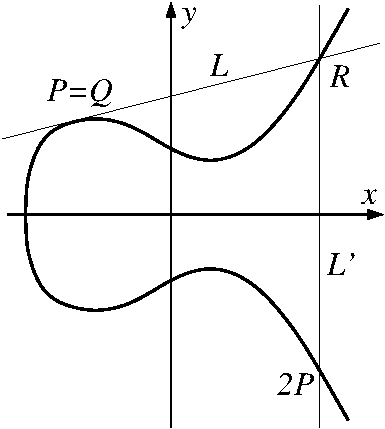
\includegraphics[scale=1.08]{ec-mult2.pdf}
\caption{Verdoppelung eines Punktes} 
\vspace{\floatsep}
\vskip +20 pt
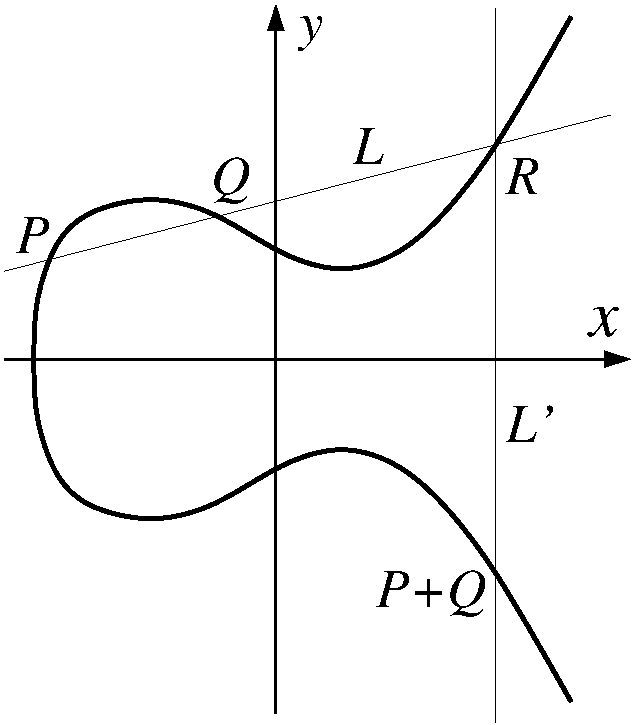
\includegraphics[scale=0.65]{ec-add.pdf}
\caption{Addition zweier verschiedener Punkte} % \footnotemark }
\end{center}
\end{figure}
% \addtocounter{footnote}{0}\footnotetext{Der Punkt $O$ kann nicht in der affinen Ebene dargestellt werden.}
\enlargethispage{+20pt}
\newpage
Zu beachten ist, dass man
${\bf E}$ folgende Bedeutungen zuordnen kann:
\begin{itemize}
   \item die Menge ${\bf E}$ der L"osungspaare $(x,y)$ einer Gleichung inklusive dem Punkt $O$ %\\[-20 pt]
   \item die Gruppe ${\bf E}$ (mit der Verkn"upfung \glqq Addition von $(x_1,y_1)$ und $(x_2,y_2)$\grqq) %\\[-20 pt]
   \item die Elliptische Kurve ${\bf E}$ (die eigentlich dasselbe wie die Gruppe ${\bf E}$ ist) %\\[-20pt]
 \end{itemize}

Da diese Bezeichnungen eigentlich alle dasselbe meinen, ist eine Unterscheidung "uber die genaue Bedeutung nur
selten n"otig.

F"ur die Kryptographie ist die Tatsache von Bedeutung, dass es f"ur sehr gro"se Zahlen extrem schwierig zu
sein scheint, aus einem gegebenem Punkt $Q$ auf einer Elliptischen Kurve festzustellen, welche beiden
Punkte addiert werden m"ussen, um $Q$ zu erhalten.

F"ur gro"se Zahlen $a, b$ und $p$ ($p$ ist zum Beispiel
mehr als $160$ Bit lang) ist der Computer ohne weiteres in der Lage, sehr schnell (in wenigen
Bruchteilen einer Sekunden) den Punkt $P$  $m$ mal hintereinander zu addieren, also den Punkt
$P + P + \cdots + P = Q$ ($m$ Summanden $P$) zu bestimmen. Statt $P + P + \cdots + P = Q$ ($m$ Summanden $P$)
schreibt man auch $mP = Q$. Hat man einen Punkt $P$ und einen Punkt $Q$, die beide auf der gleichen
Elliptischen Kurve liegen, ist allerdings kein Verfahren bekannt, das es erm"oglicht --- in
akzeptabler Zeit --- diejenige Zahl $m$ zu bestimmen (falls es diese "uberhaupt gibt), mit der $mP = Q$ gilt.
Dies wird als das \glqq Diskrete Logarithmus Problem "uber Elliptischen Kurven\grqq\ bezeichnet
(auch ECDLP\index{ECDLP} - Elliptic Curve Discrete Logarithm Problem - abgek"urzt).
\vskip +5 pt

Es ist zu beachten, dass nicht alle Elliptischen Kurven gleich sicher sind. Das bedeutet, dass man bei der
Definition einer Kurve auf die Wahl der Parameter $a$ und $b$ achten mu"s. Denn f"ur bestimmte Klassen von
Elliptischen Kurven ist es m"oglich, das ECDLP leichter zu l"osen als im allgemeinen Fall. Kryptographisch
ungeeignete Elliptische Kurven sind die sogenannten {\em anormalen} Kurven (das sind Kurven "uber ${\mathbb Z}_p$,
f"ur die die Menge ${\bf E}$ genau $p$ Elemente hat) und die {\em supersingul"aren} Kurven (das sind Kurven, f"ur die man das
Berechnen des ECDLP auf das Berechnen des \glqq normalen\grqq\ Diskreten Logarithmus in anderen endlichen K"orper
reduzieren, d.h. vereinfachen, kann). Daher gibt es kryptographisch gute und schlechte Kurven. Allerdings
kann man f"ur gegebene Parameter $a$ und $b$ mit etwas Aufwand feststellen, ob die resultierende Elliptische
Kurve kryptographisch brauchbar ist oder nicht. Die in der Kryptographie eingesetzten Kurven werden meist
von Fachleuten zur Verf"ugung gestellt. Sie gew"ahrleisten, dass die von ihnen als sicher eingestuften
Elliptischen Kurven den aktuellen Sicherheitsanforderungen gen"ugen.
\vskip +5 pt

Bei sicheren Kurven wird haupts"achlich
durch den Parameter $p$ bestimmt, wie lange es dauert, das ECDLP auf dieser Kurve zu l"osen. Je gr"o"ser der
Parameter $p$ ist, desto l"anger nimmt das L"osen des Problems in Anspruch. Von Fachleuten wird eine Bitl"ange
von "uber $200$ Bit f"ur den Parameter $p$ empfohlen. Hier wird deutlich, warum die Elliptischen Kurven so
interessant f"ur die Kryptographie sind. Denn der Parameter $p$ bestimmt auch den
Signatur-/Verschl"usselungsaufwand, der aufgewendet werden mu"s, wenn mit Elliptischen Kurven
Kryptographie betrieben wird. Die Dauer einer Schl"usselpaar-Erzeugung ist ebenfalls von
$p$ abh"angig. Daher sind kleine Werte (wenige Bits) w"unschenswert (m"oglichst schnelle Laufzeiten der Verfahren);
allerdings mu"s die geforderte Sicherheit dabei eingehalten werden. Mit einer L"ange von zum Beispiel $200$ Bit
f"ur $p$ ist eine {\em gute} Elliptische Kurve genau so sicher wie ein \index{RSA!Modul} RSA-Modul von "uber $1024$ Bit L"ange
(zumindest nach dem heutigen Forschungstand). Der Grund daf"ur ist, dass die schnellsten Algorithmen zum
L"osen des {\em Elliptische Kurven Diskreter Logarithmus} Problems eine exponentielle Laufzeit haben --- im
Gegensatz zu den subexponentiellen Laufzeiten, die die zur Zeit besten Faktorisierungsalgorithmen haben
(Zahlk"orpersieb, Quadratisches Sieb oder Faktorisieren mit Elliptischen Kurven). Daher m"ussen die
Parameter von Kryptoverfahren, die auf dem Problem {\em Faktorisieren von ganzen Zahlen} beruhen, gr"o"ser sein als
die Parameter von Kryptoverfahren, die auf dem ECDL-Problem basieren.

% --------------------------------------------------------------------------------------------------------------------
\subsubsection{Digitale-Signaturen mit Elliptischen Kurven}

Das {\em Elliptische Kurven Diskreter Logarithmus Problem}\index{Logarithmusproblem} (ECDLP) \index{ECDLP} ist die Grundlage f"ur die
Elliptische--Kurven--Kryptographie. Ausgehend von dieser Grundlage gibt es verschiedene Signaturverfahren.
Sie haben gemeinsam, wie sie die folgenden "offentlichen Parameter benutzen und wie damit der geheime und
der "offentliche Schl"ussel erzeugt werden:
\begin{itemize}
    \item Die Parameter der Elliptischen Kurve {\bf E}, das hei"st eine Primzahl $p$, die festlegt,
          "uber welchem K"orper ${\mathbb Z}_p$ die Elliptische Kurve ${\bf E}$ definiert ist, sowie die beiden
          Zahlen $a$ und $b$ aus ${\mathbb Z}_p$.
    \item Ein Punkt $G=(x,y)$, der auf der Elliptischen Kurve ${\bf E}$ liegt.
    \item Eine Primzahl $r < p$, f"ur die gilt $rG=O$ (also $r$ mal $G$ addiert ergibt das neutrale Element der
          Gruppe ${\bf E}$) und $r$ ist ein Teiler von $\#{\bf E}$ (mit $\# {\bf E}$ ist die Anzahl der Elemente in der
          Menge ${\bf E}$ gemeint). Der Punkt $G$ hat also die Ordnung $r$ und ist der Generator einer
          zyklischen Untergruppe von ${\bf E}$ mit der Ordnung $r$.
    \item Die Zahl $k = \#{\bf E}/r$ ($k$ ist der sogenannte {\em Kofaktor}).
\end{itemize}
Die eben genannten Parameter $a, b, p, G, r$ und $k$ bezeichnet man als \index{Domain-Parameter} {\em Domain}-Para\-meter. Durch sie wird
festgelegt, auf welcher Elliptischen Kurve ${\bf E}$ und in welcher zyklischen Untergruppe von ${\bf E}$ ein
Signaturverfahren \glqq eingesetzt\grqq\ wurde.

Der geheime Schl"ussel $s$ des Signaturerstellers ist eine (zuf"allige) ganze Zahl $s$ aus dem
Intervall $[1, r-1]$. Der "offentliche Schl"ussel des Signaturerstellers ist ein Punkt $W=(x,y)$ auf der
Elliptischen Kurve ${\bf E}$. "Offentlicher Schl"ussel $W$ und geheimer Schl"ussel $s$ h"angen wie folgt voneinander ab:
$W = sG$. Das hei"st durch die Domain-Parameter (insbesondere $G$) und den geheimen Schl"ussel $s$
wird der "offentliche Schl"ussel $W$ berechnet (durch $s$-malige Addition von $G$ auf ${\bf E}$). Hier wird ganz
offensichtlich von dem ECDLP Gebrauch gemacht: Kennt jemand $W$ und $G$
(sowie die anderen benutzten Domain-Para\-meter), so ist es schwierig, daraus $s$ zu berechnen
(f"ur richtig gew"ahlte Parameter scheint dies zur Zeit praktisch unm"oglich zu sein).

Um eine Signatur zu verifizieren, mu"s dem Empf"anger der Signatur folgendes bekannt sein:
\begin{enumerate}
   \item das eingesetzte Signaturverfahren,
   \item die eingesetzte Hashfunktion,
   \item die zum Signieren benutzten Domain-Parameter und
   \item der "offentliche Schl"ussel $W$ des Signaturerstellers.
\end{enumerate}


% --------------------------------------------------------------------------------------------------------------------------
\subsubsection{Faktorisieren mit Elliptischen Kurven}
\hypertarget{faktell}{}

Es gibt Faktorisierungalgorithmen, die auf Elliptischen Kurven basieren\footnote{Im Jahr 1987 stellte H.W. Lenstra\index{Lenstra 1987}
einen Faktorisierungsalgorithmus vor, der auf elliptischen Kurven basiert 
(Siehe \cite{Lenstra1987}). Die aktuell gr"o"ste mit elliptischen Kurven faktorisierte Zahl  
ist die 55 Dezimalstellen lange Zahl $629^{59}-1$, sie wurde am 6. Oktober 2001 von M. Izumi gefunden (Siehe \hyperlink{Lenstra2}{ECMNET}\index{ECMNET}).}. 
Genauer gesagt, machen sich diese Verfahren zunutze, dass man auch "uber ${\mathbb Z}_n$ ($n$ zusammengesetzte Zahl)
Elliptische Kurven definieren kann. Elliptische Kurven "uber ${\mathbb Z}_n$ bilden keine Gruppe, da es nicht zu jedem 
Punkt auf solchen Elliptischen Kurven einen inversen Punkt geben mu"s. Dies h"angt damit zusammen, dass es -- falls $n$ 
eine zusammengesetzte Zahl ist -- in ${\mathbb Z}_n$ Elemente gibt, die kein Inverses bez"uglich der Multiplikation
modulo $n$ haben. Um zwei Punkte auf einer Elliptischen Kurve "uber ${\mathbb Z}_n$ zu addieren, kann
prinzipiell genauso gerechnet werden wie auf Elliptischen Kurven "uber ${\mathbb Z}_p$. Eine Addition von zwei
Punkten (auf einer Elliptischen Kurve "uber ${\mathbb Z}_n$) scheitert aber genau dann, wenn man einen Teiler
von $n$ gefunden hat. Der Grund daf"ur ist, dass das Verfahren zum Addieren von Punkten auf Elliptischen
Kurven Elemente in ${\mathbb Z}_n$ ermittelt und zu diesen Elementen die inversen Elemente (bez"uglich der
Multiplikation modulo $n$) in ${\mathbb Z}_n$ berechnet. Dazu wird der erweiterte \index{Euklidscher Algorithmus} Euklidsche Algorithmus benutzt.
Ergibt sich nun bei der Addition zweier Punkte (die auf einer Elliptischen Kurve "uber ${\mathbb Z}_n$ liegen) ein
Element aus ${\mathbb Z}_n$, das kein inverses Element in ${\mathbb Z}_n$ hat, so gibt der erweiterte Euklidsche Algorithmus\index{Euklidscher Algorithmus!erweiterter}
einen echten Teiler von $n$ aus.

Das Faktorisieren mit Elliptischen Kurven funktioniert somit prinzipiell so: Man w"ahlt zuf"allige Kurven
"uber ${\mathbb Z}_n$, sowie zuf"allig irgendwelche Punkte (die auf diesen Kurve liegen) und addiert diese; dabei
bekommt man wieder Punkte, die auf der Kurve liegen oder findet einen Teiler von $n$. Die
Faktorisierungsalgorithmen auf Basis von Elliptischen Kurven arbeiten also probabilistisch.
Durch die M"oglichkeit, sehr viele Elliptische Kurven "uber ${\mathbb Z}_n$ zu definieren, kann man die
Wahrscheinlichkeit erh"ohen, zwei Punkte zu finden, bei deren Addition ein Teiler von $n$ gefunden wird.
Daher eigenen sich diese Verfahren auch sehr gut f"ur Parallelisierung.

% ---------------------------------------------------------------------------------------------------------------------
\subsection{Implementierung Elliptische Kurven}

CrypTool benutzt Elliptische Kurven bei der Funktion f"ur digitale Signaturen.

Implementiert sind die Basisalgorithmen f"ur Gruppenoperationen, f"ur das Erzeugen von Elliptischen
Kurven und f"ur das Ein- und Auslesen von Parametern f"ur Elliptische Kurven "uber endlichen
K"orpern mit $p$ ($p$ prim) Elementen. Die Implementierung erfolgte in ANSI C und richtete sich
nach dem Entwurf Nr.8 der Arbeitsgruppe IEEE P1363 {\em Standard Specifications for Public Key Cryptography}

{\href{http://grouper.ieee.org/groups/1363}{\tt http://grouper.ieee.org/groups/1363}}.

Implementiert sind die kryptographischen Primitive zur Signaturerzeugung und Signaturverifikation f"ur
die auf Elliptischen Kurven basierenden Varianten von Nyberg-Rueppel-Signaturen und \index{DSA} DSA-Signaturen
(nach Entwurf Nr.8 der Arbeitsgruppe IEEE P1363). Dies erfolgte in Zusammenarbeit mit der SECUDE
GmbH --- und unter Benutzung der obigen Bibliothek und des SECUDE SDK.
\index{SECUDE GmbH}

\newpage
%\addcontentsline{toc}{subsection}{Literaturverzeichnis}
\begin{thebibliography}{99999}
\addcontentsline{toc}{subsection}{Literaturverzeichnis}
	\bibitem[Lenstra1987]{Lenstra1987} H.W. Lenstra\\ \index{Lenstra 1987}
		Factoring integers with elliptic curves, Annals of Mathematics 126, pp. 649-673, 1987.
\end{thebibliography}

\section*{URLs}\addcontentsline{toc}{subsection}{URLs}

\begin{enumerate}
   \item Online-Tutorial "uber elliptische Kurven der Firma Certicom\index{Certicom}\\
		\href{http://www.certicom.com/resources/ecc_tutorial/ecc_tutorial.html}{\tt http://www.certicom.com/resources/ecc\_tutorial/ecc\_tutorial.html}
	\item Arbeitsgruppe IEEE P1363

		\href{http://grouper.ieee.org/groups/1363}{\tt http://grouper.ieee.org/groups/1363}
	\item  \hypertarget{Lenstra2} Eine informative Seite zum Faktorisieren mit elliptischen Kurven

	\href{http://www.loria.fr/~zimmerma/records/ecmnet.html}{\tt http://www.loria.fr/\~{}zimmerma/records/ecmnet.html}

	Dort findet man Literatur zum Thema Faktorisieren mit elliptischen Kurven sowie Links
zu anderen Seiten.

\end{enumerate}


\addcontentsline{toc}{section}{Index} \printindex
%
% ......................................................................................................................
%
% ~~~~~~~~~~~~~~~~~~~~~~~~~~~~~~~~~~~~~~~~~~~~~~~~~~~~~~~~~~~~~~~~~~~~~~~~~~~~~~~~~~~~~~~~~~~~~~~~~~~~~~~~~~~~~~~~~~~~~~
%

\end{document}
